\documentclass[11pt,a4paper]{article}
\usepackage[UTF8,fontset=windows]{ctex}
\usepackage{amsmath,amssymb,amsthm,mathtools}
\usepackage{lmodern}
\usepackage{graphicx}
\usepackage{tikz}
\usetikzlibrary{shapes.geometric, arrows.meta, positioning, calc, backgrounds, fit, shadows}
\usepackage{geometry}
\geometry{left=2.5cm,right=2.5cm,top=2.8cm,bottom=2.8cm}
\usepackage{xurl}
\usepackage{hyperref}
\hypersetup{
    colorlinks=true,
    linkcolor=black,
    citecolor=blue!80!black,
    urlcolor=blue!80!black
}
\usepackage{booktabs}
\usepackage{array}
\usepackage{multirow}
\usepackage[numbers,sort&compress]{natbib}
\usepackage{titlesec}
\usepackage{caption}
\captionsetup{labelsep=space,font={small,bf}}

% Custom section formatting according to Chinese journal style using titlesec
\titleformat{\section}{\raggedright\heiti\zihao{4}\bfseries}{\thesection}{1em}{}
\titleformat{\subsection}{\raggedright\heiti\zihao{5}\bfseries}{\thesubsection}{1em}{}
\titleformat{\subsubsection}{\raggedright\heiti\zihao{5}}{\thesubsubsection}{1em}{}
\titlespacing*{\section}{0pt}{1.5ex plus .2ex minus .2ex}{1ex plus .2ex}
\titlespacing*{\subsection}{0pt}{1.2ex plus .2ex minus .2ex}{0.8ex plus .2ex}
\titlespacing*{\subsubsection}{0pt}{1.0ex plus .2ex minus .2ex}{0.6ex plus .2ex}

% Theorem environments
\theoremstyle{plain}
\newtheorem{theorem}{定理}
\newtheorem*{theorem5R}{定理 5R（定理 5 的时变自回归扩展）}
\newtheorem{lemma}{引理}
\newtheorem{corollary}{推论}
\theoremstyle{definition}
\newtheorem{definition}{定义}

% Remove LaTeX default proof square box (keep only Chinese '证毕。')
\renewcommand{\qedsymbol}{}

% TikZ colors
\definecolor{navyMain}{RGB}{24, 48, 89}
\definecolor{tealMain}{RGB}{16, 124, 138}
\definecolor{coralMain}{RGB}{210, 85, 40}
\definecolor{slateGray}{RGB}{65, 80, 100}
\definecolor{cardTealBg}{RGB}{242, 251, 252}
\definecolor{cardBlueBg}{RGB}{243, 247, 254}
\definecolor{cardOrangeBg}{RGB}{255, 247, 242}
\definecolor{cardGrayBg}{RGB}{248, 250, 253}
\definecolor{panelBorderBlue}{RGB}{175, 200, 230}
\definecolor{panelBorderOrange}{RGB}{245, 190, 160}

\begin{document}

% Title (without author placeholders)
\begin{center}
    \vspace*{0.5em}
    {\zihao{2}\heiti\bfseries 传染病传播动力学的可预测视界、理论极限与实证研究} \\[1.8em]
\end{center}

% Abstract & Keywords Box
\noindent{\heiti\bfseries 摘要：}针对重大传染病前瞻预测在近临界阶段频繁遭遇精度骤降与系统性失效的理论难题，本文借鉴生态学预测视界理论范式并拓展至分支动力学，推导了前瞻预测相对均方误差在假定 (A1)--(A4) 下的可加分解，建立了预设误差容忍度 $\tau$ 下可预测视界的解析映射，并给出对数正态参数传播下的高精度数值根。研究将预测误差分解为微观人口随机性方差下界与随代际几何放大的参数推断误差，给出了负二项分支似然下的 Cram\'er--Rao 样本量门槛与有限种群临界慢化标度。基于美国疾病预防控制中心（CDC）真实周度监测数据的实证测算表明：在国家级宏观大样本聚合尺度下，大数定律使得微观人口随机性方差贡献极小（占容忍度 $\tau^2$ 的比例至多为 0.74\%），理论视界主要由推断信噪比与代间隔调控；在五个非 RSV 早期指数增长期中理论视界精确根为 7.9--21.2 周，而 RSV 2025--26 流行季因窗口累计病例数低于 Cram\'er--Rao 所需独立簇样本量（比值 2.46），其无截断数学外推根达 41.5--67.8 周，显著超出呼吸道病毒单流行季 16--20 周的物理跨度，属于模型外推假象。基于生成式预测协议的四项误差记账核算显示：已建模机制项在全部评估配置中的解释占比为 0.4\%--48.4\%，未建模结构性残差占 51.2\%--99.6\%，表明真实监测误差由外生结构性扰动主导；基于真实 CDC 监测序列的伪实时滚动前瞻基准（移动块 Bootstrap 不确定性）进一步证实实际业务操作时效被压缩至 1.8--5.3 周（Delta 穿越点为 3.5 周，Omicron 为 1.8 周，流感为 5.3 周）。本研究厘清了宏观大数平滑与微观随机硬界的分野，提出了由理论机制视界与经验业务时效构成的双层探索性基准框架，为传染病预警从盲目远期外推转向基于数理极限的理性决策提供了量化参照。

\vspace{0.8em}
\noindent{\heiti\bfseries 关键词：}传染病预测；可预测视界；分支过程；内在随机性；近临界动力学；Fisher 信息量；模型误设

\vspace{1.5em}


\section*{0\quad 引言}
\addcontentsline{toc}{section}{0\quad 引言}

重大呼吸道传染病（如新型冠状病毒感染、季节性流感及呼吸道合胞病毒感染）的周期性暴发与全球蔓延，对人群生命健康与医疗卫生体系构成了严峻挑战。在暴发早期与流行态势演化过程中，及时、可靠的前瞻性预测是公共卫生决策部门优化重症医疗资源配置、调度抗病毒药物储备以及科学部署非药物干预（NPI）措施的关键生命线。然而，流行病预测在实际业务中长期面临突出的性能衰退瓶颈：在疫情进入稳定指数上升或下降阶段时，各类预测模型通常能维持较好的拟合优度；但一旦疫情接近流行阈值（即基本再生数 $R \approx 1$ 的临界拐点）或进入多周前瞻预测，预测系统的表现便发生系统性劣化，不仅预测区间急剧发散，点预测甚至频繁出现方向性误判\citep{scarpino2019predictability, reich2019collaborative}（Scarpino 与 Petri\citep{scarpino2019predictability} 亦从信息论角度刻画了突发暴发的内在排列熵屏障）。这种在近临界状态下预测能力的断崖式退化，直接削弱了预警系统的实战效能。

为应对传染病前瞻预测的重大现实需求，计算流行病学在过去数十年间形成了四大主流建模流派：一是基于仓室生灭的机械动力学流派（如经典 SIR/SEIR 及其扩展微分方程），强调传播机理与接触结构表达；二是基于统计推断的时间序列流派（如自回归移动平均、广义相加模型及更新方程），侧重趋势平滑与概率区间标定；三是基于数据驱动的深度学习与机器学习流派（如循环神经网络、时空图注意力网络及梯度提升树），通过高维非线性特征拟合复杂流行模式；四是多模型协同与集合数据同化流派（如集合卡尔曼滤波及多机构预测集成中心）。然而，大规模真实疫情的多模型协同评估项目——包括美国 CDC FluSight 流感预测\citep{mcgowan2019collaborative, flusight2024evaluation}、RAPIDD 埃博拉多模型评估\citep{viboud2018rapidd}、登革热预测挑战\citep{johansson2019open}以及 COVID-19 协同预测中心\citep{cramer2022evaluation}——在跨越数年、数万次预测的系统评估中揭示了一个令人深思的共同瓶颈：无论是复杂的唯象动力学还是参数庞大的前沿神经网络，其在前瞻 3--4 周后的预测技能普遍发生严重衰退，甚至难以稳健超越最简单的基线外推模型\citep{suez2026baseline, lopez2024challenges}。更深层次的动力学分析表明，传染病系统在结构上存在固有的识别瓶颈：Melikechi 等\citep{melikechi2022limits}针对典型 SIR 仓室模型给出了近似分析，指出了预峰暴发爬坡期存在突出的实用不可识别性挑战（Practical Unidentifiability），即极度发散的远期预测轨迹能够在观测噪声下产生统计等效的近期拟合，造成机理推断在本质上的多解性；同时，监测网络不可避免的报告延迟与数据回填修订泄漏进一步加剧了实时预报的扰动\citep{mcdonald2021auxiliary}。尽管加权区间评分（WIS）\citep{bracher2021evaluating}等标准化工具能够对预测误差进行精细的事后度量，但现有方法论主要局限于经验性回顾评测，始终缺少直接以底层生灭动力学为起点的理论方程，无法在事前回答“某一流行阶段究竟在多大时间跨度内是理论可预测的”。

这一经验困境引出了计算流行病学领域一个悬而未决的核心科学问题：传染病传播系统是否存在独立于具体预测算法与模型结构的“内在可预测性边界”？若存在，该边界究竟由何种数理机制所决定？微观个体的随机生灭涨落、超扩散过离散特征（聚集度参数 $k$）、宏观参数推断不确定性（$\delta R$）以及外生结构性扰动，是如何交织并定量塑造这一极限的？在可预测性理论极限的探索脉络中，经典随机过程与生物数学做出了奠基性工作：Bartlett\citep{bartlett1957measles}与 Athreya 和 Ney\citep{athreya1972branching}确立了分支过程的二阶矩递推；Whittle\citep{whittle1955outcome}解析了分支过程的随机建群与灭绝概率；Castro 等\citep{castro2020predictability}论证了扩张期疫情转折点对初始微扰的敏感性；Rosenkrantz 等\citep{rosenkrantz2022fundamental}从网络图论证明了多步前瞻网络测度计算在最坏情形下具有 \#P-hard 计算复杂性（尽管在特定拓扑约束下存在多项式近似算法）；Parag 与 Donnelly\citep{parag2022fundamental} 在泊松更新框架下导出了再生数推断的 Fisher 信息量与 Cram\'er--Rao 下界；Penn 等\citep{penn2023intrinsic}基于概率母函数解析导出了代际偶然方差的递推分解。需要指出的是，“预报视界”作为首次穿越应用相关技能阈值的概念源自生态学预测研究\citep{petchey2015ecological}，分支过程框架下的预报精度分析亦可追溯至 Drake\citep{drake2006limits} 对直接传播疾病暴发预报精度的分支极限分析；Penn 等\citep{penn2023intrinsic}已区分偶然不确定性与认知不确定性并允许负二项子代分布，Parag 与 Donnelly\citep{parag2022fundamental, parag2022quantifying}给出了含噪流行曲线下的检测延迟极限。在此基础上，借鉴多源不确定性分解架构\citep{dietze2017prediction, wesselkamp2025forecast, park2020reconciling}与模型误设/参数辨识性考量\citep{king2015avoidable}，本文的贡献并非发明“阈值穿越视界”概念本身，而是其特定解析实例化：在统一负二项分支框架下，将微观生灭方差与宏观参数推断误差转化为容忍度 $\tau$ 约束下的显式视界求根方程，把五维参数 $(R, k, I_0, s, \tau)$ 映射为理论可预测时效上限，并给出其统计推断（参数化 Bootstrap）与真实监测数据的完整生成链。

针对上述关键空白，本文从多类型连续时间负二项分支过程与大数极限扩散逼近的第一性原理出发，推导出了前瞻预测相对均方误差的理论加性分解，导出了可预测视界领先阶闭式解 $h^*$ 与高阶精确数值根 $h^*_{\text{exact}}$。本文严格刻画了有限宿主种群在流行阈值附近的拟平稳扩散平稳态与临界慢化时间标度（$O(N^{1/2})$），导出了超临界判别的 Cram\'er--Rao 信息论样本量刚性下限，并构建了四项预测误差记账架构与多层公卫决策转化机制。通过对美国疾病预防控制中心（CDC）三大呼吸道传染病（COVID-19、流感、RSV）七大典型流行阶段真实序列的系统实证测算与逐周伪实时滚动样本外预测验证，本文揭示了理论机制上限与业务可操作预测时效构成的双层分析框架。

本文的结构安排如下：第 1 节系统回顾协同预测评估、分支过程、拟平稳动力学及可预测性理论边界的相关研究进展；第 2 节建立基于负二项分支过程的理论模型，给出引理 1--3 的严格数学证明，推导均方误差加性分解、闭式视界上限及核心理论定理（定理 1--5R 与推论 1--3）；第 3 节介绍高通量蒙特卡洛随机模拟验证设计与机器学习算法基准检验；第 4 节报告美国 CDC 三大呼吸道传染病典型阶段的真实视界测算、四项预测误差记账实测分解与伪实时滚动样本外评估结果；第 5 节深入探讨从理论视界到公卫预警规则的决策转化机制、健康公平性考量及研究局限性；第 6 节总结全文主要结论。

\section{研究回顾}

\subsection{协同预测项目与系统性评估}
多模型协同预测评估项目已在大规模真实疫情中完整记录了临界失效模式。FluSight 流感预测\citep{mcgowan2019collaborative}、RAPIDD 埃博拉多模型评估\citep{viboud2018rapidd}、登革热预测计划\citep{johansson2019open}与 COVID-19 协同预测中心\citep{cramer2022evaluation}系统性比较了数十个团队的模型表现，一致发现在近临界阶段模型预测技能普遍降至甚至低于简单的基线外推模型，但始终缺少统一的动力学方程将流行病学参数与可达精度极限直接相连。近期，Mathis 等\citep{flusight2024evaluation}对 FluSight 多季流感协同预测进行了系统性多模型基准评估，证实预测模型在疫情快速变化期与转折拐点处精度显著承压；White 与 Le{\'o}n\citep{white2026forecastability}进一步探讨了不同病原体时间序列可预测性测度的内在差异。Suez 与 Fox\citep{suez2026baseline}以及 Lopez 等\citep{lopez2024challenges}深入论证了基线模型设计（如持续性外推对局部趋势外推）对预测技能比评估的决定性影响，揭示了协同预报中心模型在 3--4 周后普遍落后于基准外推的经验瓶颈。同时，McDonald 等\citep{mcdonald2021auxiliary}明确指出真实预测评估需高度警惕固化数据（Finalized Vintage）带来的回填修订泄漏（Backfill Leakage）。然而现有协同评估方法论（如加权区间评分 WIS\citep{bracher2021evaluating}）通常侧重于事后评测，缺少直接源自底层生灭动力学的第一性原理理论视界 $h^*$ 作为事前分析基准。本文推导的视界公式为量化经验预测技能衰减提供了理论物理参照。

\subsection{分支过程与更新方程}
分支过程与更新方程作为传染病动力学推断的基石具有深厚理论渊源。负二项子代分布的 Galton--Watson 过程\citep{harris1963branching, athreya1972branching, jagers1975branching}与连续时间更新方程\citep{wallinga2004different, wallinga2007generation, cori2013framework}为实时 $R_t$ 估计\citep{abbott2020epinow2, gostic2020practical}与早期增长率推断\citep{bettencourt2008real}提供了标准的统计似然基础。近年来，研究者广泛将离散度参数 $k$ 作为超扩散程度的度量指标\citep{lloyd-smith2005superspreading, endo2020overdispersion}，并深入探讨了过度离散对再生数推断精度的决定性影响\citep{ho2023simultaneous, nemcova2026unjustified}。Hébert-Dufresne 等\citep{hebert-dufresne2020beyond} 较早基于负二项分支母函数框架探讨了过度离散度 $k$ 对终末暴发规模与入侵概率不确定性的决定性影响，但其侧重于终末静态特征，尚未建立多步前瞻动态误差方差的加性分解与定量预测视界 $h^*$ 的闭式求解映射。在不确定性解耦方面，Penn 等\citep{penn2023intrinsic}基于概率母函数解析导出了偶然方差随代际递推的更新方程，显式将偶然方差分解为感染期、子代分布与历史传播三项机制分量（其式 9）；而本文聚焦于偶然不确定性与认知参数不确定性之间的跨源关系，在假定 (A4) 独立性下推导出了微观生灭方差下界与宏观参数推断误差的严格加性均方误差分解（式 \ref{eq:relmse_decomp}），直接给出了均方误差与预测视界的闭式解析映射，两者在分析维度上正交互补。此外，经典的代间隔正向链接\citep{park2021forward}、再生数估计\citep{fraser2007estimating}及简单更新外推模型\citep{nouvellet2018simple}侧重于即期点估计，本文则将分支过程结构拓展至多步前瞻预测的理论极限分析。

\subsection{临界现象与拟平稳动力学}
统计物理中的临界相变与灭绝动力学为描述近临界流行病过程提供了精细的随机分析工具。分支过程的拟平稳分布（Quasi-Stationary Distribution, QSD）\citep{darroch1965quasi}、临界慢化现象\citep{kessler2007extinction}、Logistic 扩散逼近\citep{ethier1986markov}与动力学渗透理论\citep{grassberger1983critical}刻画了有限种群中当 $|\varepsilon|=|R-1| \ll 1$ 时的长尾涨落与建群概率（Establishment Probability）。Britton 与 Tomba\citep{britton2019estimation}分析了阈值附近的参数估计偏差。有限种群阈值的生物数学争论\citep{lloydsmith2005should}指出随机干扰抹平了确定性 $R_0 = 1$ 的分界线；N{\aa}sell\citep{nasell1999quasi}与 Dolgoarshinnykh 和 Lalley\citep{dolgoarshinnykh2006critical}严格推导了随机流行病模型在临界态附近的扩散标度与拟平稳渐近。在生态与流行病早期预警信号（Early Warning Signals, EWS）领域，O'Regan 和 Drake\citep{oregan2013theory} 与 Southall 等\citep{southall2021early} 深入探讨了临界相变点附近的拟平稳态与临界慢化方差放大机制；本文定理 3 则进一步将 $O(N^{1/2})$ 弛豫时间发散标度严格解析映射为可预测视界的极限收缩边界。

\subsection{传染病预测中的机器学习理论边界}
近年来，机器学习与深度学习被广泛应用于传染病预测任务，从流感预测基准\citep{reich2019collaborative, ray2023comparing}到多源正则化机器学习\citep{colubri2019machine}与深度自回归网络\citep{salinas2020deepar}。然而现有文献大多聚焦于经验性能对比（即“哪个模型在特定数据集上表现更优”），极少追问其相对于理论最小均方误差下界的位置。LightGBM 等梯度提升树\citep{ke2017lightgbm}与多层感知机（MLP）虽展现出强大的非线性拟合能力，但在无偏数据生成机制下能否突破理论辨识极限此前缺乏严格测试。

值得注意的是，现有关于流行病预测理论极限的研究主要沿三条独立路径展开：第一条是确定性动力系统路径，例如 Castro 等\citep{castro2020predictability}论证了流行病峰值转折点对初始条件敏感性的不可预测性约束；第二条是网络图论与计算复杂性路径，Rosenkrantz 等\citep{rosenkrantz2022fundamental}证明了即便已知完全网络结构与真实动力学参数，计算未来多步宏观发病测度仍属 \#P-hard 难题，确立了算法计算效率层面的根本极限；第三条是信息论与随机推断路径，例如 Parag 与 Donnelly\citep{parag2022fundamental} 在泊松更新模型下导出了有效再生数的 Fisher 信息量与 Cram\'er--Rao 界，揭示了实时追踪复发风险的信息提取下界，而 Moran 等\citep{moran2016epidemic}系统阐释了人类自适应行为与报告延迟对预测形成的不可约扰动。本文继承并拓展了随机过程与信息论路径，将子代模型推广至负二项过度离散情形，并在统一的负二项分支框架中导出了连接五维动力学参数 $(R, k, I_0, \delta R, \tau)$ 到定量预测视界的显式表达，为判断算法改进是逼近了模型内在的推断上限还是仅在优化局部拟合提供了参照基准。

需要明确区分两类本质不同的“可预测性理论极限”概念：一类是基于时间序列信息熵与非线性相空间重构的内在可预测性（entropy-based intrinsic predictability，如 Song 等\citep{song2010limits}对人类移动轨迹的香农熵界、Scarpino 与 Petri\citep{scarpino2019predictability}对流行病时间序列排列熵与 Lyapunov 指数的测算、以及 White 与 Le{\'o}n\citep{white2026forecastability}对跨病种可预测性的比较），该路径回答的是“观测时间序列本身蕴含多少可预测信息与混沌不规则性”；另一类则是基于统计推断与信息几何的估计精度理论极限（estimation-theoretic precision limits，如 Parag 与 Donnelly\citep{parag2022fundamental, parag2022quantifying}的一系列开创性工作），回答的是“在给定的微观随机生成模型族下，有限监测样本能将关键动力学参数推断至何种最小均方误差”。本文的研究路径严格属于后者：我们并非度量无模型假定下的全序列时间序列熵，而是在负二项分支过程的微观生成机制下，以 Fisher 信息矩阵与 Cram\'er--Rao 下界刻画参数推断精度地板，进而通过误差传播推导宏观前瞻预测视界的理论上限。

\section{理论与方法}

\subsection{数据来源与预处理}\label{sec:data}
为实证检验理论推导在真实暴发情境中的适用性，本文采用了美国疾病预防控制中心（CDC）公开发布的国家级周度聚合监测序列（数据访问快照为 2026 年 3 月公开版）。监测目标序列定义如下：COVID-19 采用 COVID Data Tracker 国家级每周确诊发病数（Confirmed Weekly Cases，数据集 \texttt{pwn4-m3yp}，覆盖 Delta 与 Omicron 阶段）；在 2023 年 5 月 11 日联邦突发公共卫生事件（PHE）到期导致确诊病例序列停报后，JN.1 流行期（2023-W48 至 2024-W02）采用 CDC 国家医疗安全网络（NHSN）周度呼吸道住院监测指标；季节性流感采用 FluView 临床实验室网络（ICLS）确诊阳性标本周数（\texttt{ICL\_NREVSS\_Clinical\_Labs.csv}）；RSV 采用 NREVSS 实验室 PCR 检测阳性原始周计数（数据集 \texttt{rgnm-fkqb}）。实证分析严格覆盖七大典型流行阶段：COVID-19 Delta 暴发期（2021-07-03 至 2021-07-31）、Omicron 达峰期（2021-12-04 至 2022-01-01）、JN.1 流行期（2023-12-16 至 2024-01-13）；季节性流感 2022--23 流行季（2022-10-08 至 2022-11-05）、2024--25 流行季（2024-11-23 至 2024-12-21）；RSV 2024--25 流行季（2024-11-09 至 2024-12-07）及 2025--26 流行季（2025-11-08 至 2025-12-06）。（注：2025 年 10 月至 11 月联邦政府停摆期间的监测盲区均经 CDC 事后回填，历史回测基于回填固化后的最终序列 Finalized Data Vintage，作为评估理论可预测性上限的无损基准，但不代表实时初报条件下的可操作性能。）本分析的直接输入为三个经整理的国家级周度聚合序列文件（SHA-256 校验和与版本标识在代码仓库清单 \texttt{manifest} 中存档），全部参数估计、区间生成、表格与图件均由统一脚本链从该输入出发自动生成；原始 CDC 数据源地址、检索日期与整理脚本随代码一并开源。数据预处理以各阶段起步期连续 4 周数据作为推断窗口，采用滑动窗口对数线性回归估计净增长率与再生数 $R$ 及其标准误，结合负二项二阶矩法求解宏观过度离散度 $k_{\text{agg}}$。关于核心参数的口径定义与敏感性规范如下：
\begin{enumerate}
\item \textbf{初始发病规模 $I_0$ 的口径定义与微弱敏感性}：在表~\ref{tab:horizons} 中，$I_0$ 采用推断窗口内周度报告计数的算术平均值（如 COVID-19 Delta 阶段为 28,347，Omicron 为 66,275），其量纲为“周报告病例数”，而非未平滑的单日发病水平（在 CDC 数据集 \texttt{pwn4-m3yp} 中对应 5 周窗口累计确诊数分别为 141,735 与 331,377）。理论与数值灵敏度分析表明，由于国家级大样本下群体内在方差地板 $\text{CV}_\infty^2 = \frac{1+R/k_{\text{agg}}}{I_0(R-1)} \le 0.002$，远低于预设容忍度方差 $\tau^2 = 0.25$，因此即便将 $I_0$ 替换为窗口累计数或其它合理口径，视界精确根 $h^*_{\text{exact}}$ 的相对变动幅度仍小于 0.01\%，实证视界结论对 $I_0$ 选取口径具有数值刚性。
\item \textbf{代间隔 $\mu_g$ 的文献区间与敏感性}：Delta 阶段基准值取文献报道的内在代间隔（Intrinsic Generation Time）4.7 天（95\% CrI 4.1--5.6 天）\citep{hart2022generation}；作为对比，同篇文献报告的家庭接触代间隔（Household Generation Time）为 3.2 天（95\% CI 2.5--4.2 天）。当代间隔在文献报道区间 3.2--5.6 天内变动时，Delta 理论视界（以周计）相应按 $\mu_g/7$ 的比例线性缩放（基准 21.2 周对应区间约 14.4--25.3 周）；RSV 在南非家户基准 8.4 天\citep{cohen2024respiratory}与日托高频接触敏感性对照 3.2 天之间变动时，视界相应大幅平移。这表明世代视界 $h^*_{\text{gen}}$ 构成了跨病原体客观比较的内在尺度，而日历周视界严格正比于代间隔大小。
\item \textbf{代际时间离散化与日历周尺度映射（$\mu_g / 7$）}：经典 Galton--Watson 分支过程以感染世代（generation）为自然演化步长 $h \in \mathbb{N}$，其均值与方差递推严格作用于代际尺度；而公共卫生监测业务以自然周（7 天）为聚合周期。设周度对数发病回归斜率为每周对数增长率 $b_{\text{week}}$（标准误 $\text{SE}(b_{\text{week}})$，取标准 OLS 斜率标准误，自由度 $W-2$），则代际尺度（$\Delta_g = \mu_g/7$ 周）下的对数增长率为 $b_{\text{gen}} = \Delta_g b_{\text{week}}$，其标准误经 Delta 方法传播为 $s_{\text{gen}} = \Delta_g\,\text{SE}(b_{\text{week}})$，再生数 $R = \exp(b_{\text{gen}})$。参数外推项 $P(h)$ 仅通过无量纲乘积 $h \cdot s_{\text{gen}}$ 进入视界方程，而 $h_{\text{gen}} s_{\text{gen}} = h_{\text{周}} \text{SE}(b_{\text{week}})$，因此“直接在周尺度上求解视界方程”与“在代际尺度求解后乘以 $\mu_g/7$ 折算为周”两种自洽口径给出完全相同的日历周视界（本节数值验证误差 $< 0.01\%$），视界的标度结构由推断信噪比唯一决定，与折算路径无关。
\end{enumerate}
目标容忍度设为 $\tau = 0.5$（对应相对均方根误差 50\%），采用 2,000 次参数化 Bootstrap 重抽样（固定随机种子 20260807）评估动力学参数与视界置信区间：每个 Bootstrap 复制样本在拟合直线周围重抽样对数尺度残差、重新拟合斜率及其标准误、重新以二阶矩法估计 $k^*$ 与 $I_0^*$，并重新求解视界方程，取 2.5\%--97.5\% 分位数区间。

\subsection{模型设定与基础引理证明}

本文在微观层面采用标准 Galton--Watson 负二项分支过程作为基础数据生成模型，图~\ref{fig:framework_cn}系统展示了从双源随机性输入到相对均方误差可加分解，再到预测视界闭式解与核心推论的理论推导脉络。

\begin{figure}[htbp]
\centering
\resizebox{0.96\textwidth}{!}{%
\begin{tikzpicture}[
    >=Stealth,
    font=\sffamily,
    card/.style={
        rectangle, rounded corners=6pt, draw=#1, fill=white, line width=1.1pt,
        inner sep=8pt, align=center, drop shadow={opacity=0.07, shadow xshift=1pt, shadow yshift=-1.5pt}
    },
    subcard/.style={
        rectangle, rounded corners=4pt, draw=#1, line width=0.8pt,
        inner sep=5pt, align=center
    },
    panel/.style={
        rectangle, rounded corners=8pt, draw=#1, line width=0.9pt, dashed, inner sep=10pt, fill opacity=0.35
    },
    arrow/.style={
        ->, line width=1.3pt
    }
]

% 1. TIER 1: INPUT NOISE SOURCES
\node[card=tealMain, fill=cardTealBg, text width=6.3cm] (demo) {
    \textbf{\large\color{tealMain} 群体内在随机性（微观统计涨落）}\\[4pt]
    \footnotesize 生成机制：负二项分支过程 (子代 $\sim \text{NB}(R, k)$)\\[4pt]
    \textbf{\small 不可约方差下界（引理 2 / 定理 1）：}\\[3pt]
    $\text{CV}^2(h) = \dfrac{(1+R/k)(1-R^{-h})}{I_0(R-1)} \xrightarrow{h\to\infty} \dfrac{1+R/k}{I_0(R-1)}$
};

\node[card=navyMain, fill=cardBlueBg, text width=6.3cm, right=1.2cm of demo] (param) {
    \textbf{\large\color{navyMain} 参数不确定性（外在推断误差）}\\[4pt]
    \footnotesize 观测推断：监测窗口估计量 $\hat{R} \sim \mathcal{N}(R, \delta R^2)$\\[4pt]
    \textbf{\small 几何级放大项（引理 3）：}\\[3pt]
    $P(h) = \dfrac{\mathbb{E}[(\hat{R}^h - R^h)^2]}{R^{2h}} \approx \left(\dfrac{h\,\delta R}{R}\right)^2$
};

% 2. TIER 2: ORTHOGONAL ERROR DECOMPOSITION
\node[card=slateGray, fill=cardGrayBg, text width=12.8cm, below=1.5cm of $(demo.south)!0.5!(param.south)$] (decomp) {
    \textbf{\large\color{navyMain} 相对均方误差理论加性分解（定理 1 与单调性定理 2）}\\[6pt]
    \Large $\text{relMSE}^2(h) = \underbrace{\text{CV}^2(h)}_{\text{\normalsize 内在随机性方差下界}} + \underbrace{P(h)}_{\text{\normalsize 参数不确定性放大}} \le \tau^2$\\[5pt]
    \small\color{slateGray} （在分支过程与无偏估计独立性假定下正交无交叉项，且随前瞻步长 $h$ 严格单调递增）
};

% 3. TIER 3: HORIZON CEILING & LIMIT THEOREMS
\node[card=coralMain, fill=cardOrangeBg, text width=13.8cm, below=2.6cm of decomp.south] (horizon) {
    \textbf{\Large\color{coralMain} 理论可预测视界上限与数理界限（$h^*$）}\\[7pt]
    
    \begin{tikzpicture}[node distance=0.25cm]
        \node[subcard=coralMain, fill=white, text width=6.3cm, inner sep=4.5pt] (hmain) {
            \textbf{\small\color{coralMain} 主视界闭式公式（$R > 1$ 超临界）}\\[3pt]
            \scalebox{0.85}{$\boxed{\rule[-7pt]{0pt}{20pt}\, h^*_{\text{周}} \approx \dfrac{\mu_g}{7} \cdot \dfrac{R}{\delta R}\sqrt{\tau^2 - \dfrac{1+R/k}{I_0(R-1)}} \,}$}\\[3pt]
            \scriptsize （$\tau$ 为目标相对误差容忍度）
        };
        \node[subcard=coralMain, fill=white, text width=6.3cm, inner sep=4.5pt, right=0.25cm of hmain] (hcrit) {
            \textbf{\small\color{coralMain} 近临界正根解析解（推论 1：$R \to 1$）}\\[3pt]
            \scalebox{0.85}{$\boxed{\rule[-7pt]{0pt}{20pt}\, h^*_{\text{gen}} = \dfrac{\sqrt{b^2+4\delta R^2\tau^2}-b}{2\delta R^2} \,}$}\\[3pt]
            \scriptsize （其中 $b = \dfrac{1+1/k}{I_0}$ 为初始群体离散项）
        };
    \end{tikzpicture}\\[8pt]
    
    \begin{tikzpicture}[node distance=0.25cm]
        \node[subcard=coralMain, fill=white, text width=3.8cm, inner sep=4.5pt] (t3) {
            \textbf{\color{coralMain} 近临界相变特征 (定理 3)}\\[2pt]
            \scriptsize 拟平稳扩散涨落主导\\
            $|\varepsilon| \lesssim O(N^{-1/2}),\ h^* \to 0$\\
            推论 2 建群率 $s \approx \frac{2\varepsilon}{R(1+R/k)}$
        };
        \node[subcard=coralMain, fill=white, text width=3.8cm, inner sep=4.5pt, right=0.25cm of t3] (t4) {
            \textbf{\color{coralMain} 信息论辨识下限 (定理 4)}\\[2pt]
            \scriptsize Cramér--Rao 最小病例数\\
            $C \ge \frac{R^2(1/R+1/k)}{\varepsilon^2} \approx 231$\\
            80\% 功效需 $C \ge 1,428$
        };
        \node[subcard=coralMain, fill=white, text width=3.8cm, inner sep=4.5pt, right=0.25cm of t4] (t5) {
            \textbf{\color{coralMain} 四项完全实测记账 (定理 5/5R)}\\[2pt]
            \scriptsize 四项描述性误差记账\\
            $\text{relMSE}^2 = \text{CV}^2 + \mathcal{E}_{\text{drift}} + P$\\
            $+ \mathcal{E}_{\text{misspec}}$
        };
    \end{tikzpicture}
};

% 4. CONNECTING FLOW ARROWS
\draw[arrow, draw=tealMain] (demo.south) -- (demo.south |- decomp.north)
    node[midway, left=2pt, font=\bfseries\small\color{tealMain}] {内在机制贡献};

\draw[arrow, draw=navyMain] (param.south) -- (param.south |- decomp.north)
    node[midway, right=2pt, font=\bfseries\small\color{navyMain}] {外在推断贡献};

\node[fill=white, inner sep=3.5pt, rounded corners=3pt, draw=coralMain, line width=0.8pt, font=\bfseries\small\color{coralMain}, below=0.35cm of decomp.south] (critBadge) {首次达到目标误差容忍度 $\text{relMSE}(h^*) = \tau$};

\draw[arrow, line width=1.8pt, draw=coralMain] (decomp.south) -- (critBadge.north);
\draw[arrow, line width=1.8pt, draw=coralMain] (critBadge.south) -- (horizon.north);

% 5. BACKGROUND CONTAINERS
\begin{scope}[on background layer]
    \node[panel=panelBorderBlue, fill=cardBlueBg, fit=(demo) (param), 
          label={[anchor=south west, font=\bfseries\small\color{navyMain}, xshift=4pt, yshift=2pt]north west:【阶段 I：双源随机性底层生成机制】}] {};
          
    \node[panel=panelBorderOrange, fill=cardOrangeBg, fit=(horizon), 
          label={[anchor=south west, font=\bfseries\small\color{coralMain}, xshift=4pt, yshift=2pt]north west:【阶段 II：理论界限定量输出与公卫决策基准】}] {};
\end{scope}

\end{tikzpicture}%
}
\caption{\textbf{传染病传播动力学与预测视界理论推导原理图。}展示双源随机性输入（群体内在随机性方差下界与外在参数推断放大）、预测均方误差可加分解（定理 1 与单调性定理 2，在假定 (A4) 下交叉项消失）以及由此导出的理论可预测视界 $h^*$（含超临界闭式与近临界推论 1 解析解）和核心理论推论（定理 3 临界慢化坍塌、定理 4 信息论辨识下限与定理 5/5R 时变误差记账）。}
\label{fig:framework_cn}
\end{figure}

模型设立以下标准动力学与统计推断假定：
\begin{itemize}
\item[(A1)] 子代分布：各感染个体产生的二代病例数独立同分布服从负二项分布 $\text{NB}(R, k)$，均值为基本再生数 $R$，离散度为 $k$，单代子代方差 $\sigma^2 = R + R^2/k$。
\item[(A2)] 传播稳定性：在预测视界 $h$ 内 $R$ 保持恒定（时变与漂移推广见定理 5 与定理 5R）。
\item[(A3)] 时间尺度：平均代间隔为 $\mu_g$，代际预测步长 $h$ 对应的时间跨度为 $T = \mu_g h$。
\item[(A4)] 统计独立性：监测窗口参数估计量 $\hat{R}$ 条件独立于预测期内的微观随机传播实现。
\end{itemize}

以下给出分支过程均值与方差的一阶及二阶矩递推引理及其严格证明。

\begin{lemma}[分支过程两阶段矩递推]\label{lem:branch_moments}
设初始发病人数为 $Z_0 = I_0$，在假定 (A1) 下，第 $h$ 代新发感染人数（发病规模）$Z_h$ 的期望与方差分别为：
\begin{equation}
\mathbb{E}[Z_h] = I_0 R^h,
\end{equation}
\begin{equation}
\text{Var}(Z_h) = I_0 \sigma^2 R^{h-1} \frac{R^h - 1}{R - 1}, \quad (R \neq 1).
\label{eq:lem1_var}
\end{equation}
\end{lemma}

\begin{proof}
根据经典 Galton--Watson 分支过程理论\citep{athreya1972branching}，第 $n$ 代的新发感染人数 $Z_n$ 可严格表示为第 $n-1$ 代全部感染个体所产生子代病例数的随机加和，即
\begin{equation}
Z_n = \sum_{j=1}^{Z_{n-1}} X_{n-1, j},
\end{equation}
其中随机变量序列 $\{X_{n-1, j}\}$ 在个体间独立同分布，均服从负二项分布 $\text{NB}(R, k)$，其一阶矩为基本再生数 $\mathbb{E}[X] = R$，二阶方差为 $\text{Var}(X) = \sigma^2 = R + R^2/k$。

首先求解一阶期望。根据全期望公式（Law of Total Expectation），对前一代发病规模 $Z_{n-1}$ 取条件期望，可得
\begin{equation}
\mathbb{E}[Z_n \mid Z_{n-1}] = \sum_{j=1}^{Z_{n-1}} \mathbb{E}[X_{n-1, j}] = R Z_{n-1}.
\end{equation}
对上述等式两端取无条件数学期望，即有 $\mathbb{E}[Z_n] = R \mathbb{E}[Z_{n-1}]$。结合初始发病人数的确定性条件 $\mathbb{E}[Z_0] = I_0$，通过一阶齐次差分递推，直接解得第 $h$ 代的期望发病规模为 $\mathbb{E}[Z_h] = I_0 R^h$。

进而求解二阶方差。根据全方差分解公式（Law of Total Variance），第 $n$ 代发病人数的方差可正交分解为条件期望的方差与条件方差的期望两部分：
\begin{align}
\text{Var}(Z_n) &= \mathbb{E}[\text{Var}(Z_n \mid Z_{n-1})] + \text{Var}(\mathbb{E}[Z_n \mid Z_{n-1}]) \notag \\
&= \mathbb{E}\left[\sum_{j=1}^{Z_{n-1}} \text{Var}(X_{n-1, j})\right] + \text{Var}(R Z_{n-1}) \notag \\
&= \sigma^2 \mathbb{E}[Z_{n-1}] + R^2 \text{Var}(Z_{n-1}) \notag \\
&= \sigma^2 I_0 R^{n-1} + R^2 \text{Var}(Z_{n-1}).
\end{align}
记序列 $V_n = \text{Var}(Z_n)$，则上述关系构成关于 $V_n$ 的一阶非齐次线性差分方程。为求解该递推关系，将方程两端同除以几何因子 $R^{2n}$，整理可得相邻两代的差分形式：
\begin{equation}
\frac{V_n}{R^{2n}} - \frac{V_{n-1}}{R^{2(n-1)}} = \frac{\sigma^2 I_0}{R^{n+1}}.
\end{equation}
利用初始无观测方差条件 $V_0 = \text{Var}(I_0) = 0$，对指标 $n = 1, 2, \dots, h$ 实施伸缩求和（Telescoping Sum）：
\begin{equation}
\frac{V_h}{R^{2h}} = \sigma^2 I_0 \sum_{n=1}^h R^{-(n+1)} = \frac{\sigma^2 I_0}{R^2} \cdot \frac{R^{-1}(1 - R^{-h})}{1 - R^{-1}} = \frac{\sigma^2 I_0 (R^h - 1)}{R^{h+1}(R - 1)}.
\end{equation}
将两端同乘以 $R^{2h}$，即严格导出非临界状态（$R \neq 1$）下第 $h$ 代发病规模的二阶方差解析式：
\begin{equation}
\text{Var}(Z_h) = I_0 \sigma^2 R^{h-1} \frac{R^h - 1}{R - 1}.
\end{equation}
证毕。
\end{proof}

\begin{lemma}[群体内在变异系数与方差下界]\label{lem:cv_floor}
第 $h$ 代发病人数的相对方差（即变异系数平方 $\text{CV}^2(h)$）满足严格闭式解：
\begin{equation}
\text{CV}^2(h) = \frac{\text{Var}(Z_h)}{(\mathbb{E}[Z_h])^2} = \frac{(1 + R/k)(1 - R^{-h})}{I_0(R - 1)},
\label{eq:cv_floor}
\end{equation}
该相对方差从初始状态 $\text{CV}^2(0)=0$ 出发，随预测前瞻步长 $h$ 严格单调递增。在单代首步（$h=1$）处，其严格取值为 $\text{CV}^2(1) = \frac{1+R/k}{I_0 R}$；当步长无限延伸（$h \to \infty$）时，收敛至不可约的渐近方差饱和极限 $\text{CV}^2_\infty \equiv \frac{1 + R/k}{I_0(R - 1)}$。在近临界极限（$R \to 1$）下，该式连续延拓为线性累积形式 $h(1+1/k)/I_0$。
\end{lemma}

\begin{proof}
根据变异系数平方的定义，将引理 1 导出的均值与方差表达式代入，并结合负二项子代方差展开式 $\sigma^2 = R(1 + R/k)$ 进行代数化简：
\begin{align}
\text{CV}^2(h) &= \frac{I_0 R(1 + R/k) R^{h-1} \frac{R^h - 1}{R - 1}}{(I_0 R^h)^2} \notag \\
&= \frac{I_0 (1 + R/k) R^h (R^h - 1)}{I_0^2 R^{2h} (R - 1)} \notag \\
&= \frac{(1 + R/k)(1 - R^{-h})}{I_0(R - 1)}.
\end{align}
在超临界传播体制（$R > 1$）下，几何衰减项 $R^{-h}$ 随 $h$ 严格单调递减并趋于零，因此分子项 $1 - R^{-h}$ 随步长严格单调递增并趋于 1，从而直接证明了相对方差随步长的单调性与渐近饱和极限 $\text{CV}^2_\infty$。

在考察阈值附近的近临界动力学（$R \to 1$）时，由于分母项 $R - 1 \to 0$ 且分子项 $1 - R^{-h} \to 0$，式 (\ref{eq:cv_floor}) 呈现 $0/0$ 型未定式。根据洛必达法则（L'H\^opital's Rule），分别对连续变量 $R$ 求偏导数：
\begin{equation}
\lim_{R \to 1} \frac{1 - R^{-h}}{R - 1} = \lim_{R \to 1} \frac{\frac{d}{dR}(1 - R^{-h})}{\frac{d}{dR}(R - 1)} = \lim_{R \to 1} \frac{h R^{-h-1}}{1} = h.
\end{equation}
将该极限代入式 (\ref{eq:cv_floor})，即有 $\lim_{R \to 1} \text{CV}^2(h) = \frac{h(1 + 1/k)}{I_0}$。该解析结果与直接在 $R=1$ 条件下对单代负二项相对方差 $(1+1/k)/I_0$ 进行 $h$ 步独立离散累加的结果完全吻合，证明了系统在临界阈值附近的解析连续性。
证毕。
\end{proof}

\begin{lemma}[参数不确定性的几何级放大项]\label{lem:param_amplification}
在流行病学参数推断中，对数连接广义线性回归或更新方程框架下，对数再生数满足渐近正态性 $\log \hat{R} \sim \mathcal{N}(\log R, s^2)$，其中 $s = \delta R / R$ 为相对标准误，即估计量服从对数正态分布。在假定其条件独立于预测期微观过程（假定 (A4)）的前提下，参数估计误差导致的相对均方误差贡献项为：
\begin{equation}
P(h; R, \delta R) = \frac{\mathbb{E}[(I_0 \hat{R}^h - \mathbb{E}[Z_h])^2]}{(\mathbb{E}[Z_h])^2} = \frac{\mathbb{E}[(\hat{R}^h - R^h)^2]}{R^{2h}} = \mathbb{E}\left[\left(\frac{\hat{R}}{R}\right)^{2h}\right] - 2\,\mathbb{E}\left[\left(\frac{\hat{R}}{R}\right)^{h}\right] + 1.
\end{equation}
由对数正态矩公式 $\mathbb{E}[Y^m] = \exp(\tfrac{1}{2} m^2 s^2)$（$Y = \hat{R}/R$ 服从对数尺度居中的对数正态分布），该项存在精确闭式解：
\begin{equation}
P(h; s) = \exp\!\left(2 h^2 s^2\right) - 2 \exp\!\left(\tfrac{1}{2} h^2 s^2\right) + 1.
\label{eq:param_amplification}
\end{equation}
当相对累积参数误差较小（$h s \ll 1$）时，对式 (\ref{eq:param_amplification}) 实施一阶 Delta 线性化展开，可得领先阶解析近似：
\begin{equation}
P(h; R, \delta R) \approx \left(\frac{h\,\delta R}{R}\right)^2.
\end{equation}
需要指出的是，式 (\ref{eq:horizon_cn}) 的闭式解正是基于该一阶近似导出。在目标容忍度截断点（$\tau=0.5$）处，实证阶段的无量纲累积不确定性 $h s$ 约为 0.43（见第 4 节表~\ref{tab:horizons}），此时由于指数函数的严格凸性，一阶近似相较于按式 (\ref{eq:param_amplification}) 求解的精确数值根 $h^*_{\text{exact}}$ 存在约 16.7\%--18.0\% 的系统性乐观偏置。因此，一阶闭式解 $h^*_{\text{approx}}$ 提供了参数敏感性与量纲标度的解析基准，而在高精度业务场景中，应以精确根 $h^*_{\text{exact}}$ 为准。
\end{lemma}

\begin{proof}
为导出参数估计误差随前瞻步长的传递规律，定义非线性映射函数 $f(r) = r^h$。在对数正态估计模型下 $Y = \hat{R}/R$ 服从对数尺度 $s$ 的对数正态分布，且对任意实数 $m$ 有对数正态矩公式 $\mathbb{E}[Y^m] = \exp(\tfrac{1}{2} m^2 s^2)$。将 $\mathbb{E}[(\hat{R}^h - R^h)^2]/R^{2h} = \mathbb{E}[Y^{2h}] - 2\mathbb{E}[Y^h] + 1$ 依次代入，即得精确闭式
\begin{equation}
P(h; s) = \exp\!\left(2 h^2 s^2\right) - 2 \exp\!\left(\tfrac{1}{2} h^2 s^2\right) + 1.
\end{equation}
当 $h s \ll 1$ 时，对 $\hat{R}$ 在基准点 $R$ 处实施一阶泰勒展开 $f(\hat{R}) \approx R^h + h R^{h-1}(\hat{R}-R)$，利用 $\mathbb{E}[(\hat{R}-R)^2] = \delta R^2$，可得 $\mathbb{E}[(\hat{R}^h - R^h)^2] \approx h^2 R^{2h-2} \delta R^2$；两端同除以 $R^{2h}$，即严格导出领先阶相对参数误差项的闭式近似 $P(h; R, \delta R) \approx (h\,\delta R/R)^2$。
证毕。
\end{proof}

\subsection{相对均方误差分解与预测视界定理}

\begin{theorem}[预测相对均方误差的可加分解与可预测视界映射]\label{thm:horizon}
在假定 (A1)--(A4) 下，前瞻点预测 $\hat{Z}_h = I_0 \hat{R}^h$ 的相对均方误差满足如下可加分解（在 (A4) 独立性下交叉项严格消失；若无 (A4)，则需补充交叉协方差项 $-2\,\text{Cov}(I_0\hat{R}^h - \mathbb{E}[Z_h],\, Z_h - \mathbb{E}[Z_h])/\mathbb{E}[Z_h]^2$）：
\begin{equation}
\text{relMSE}^2(h) = \frac{\mathbb{E}[(\hat{Z}_h - Z_h)^2]}{(\mathbb{E}[Z_h])^2} = \text{CV}^2(h) + P(h; s) = \frac{(1+R/k)(1-R^{-h})}{I_0(R-1)} + P(h; s),
\label{eq:relmse_decomp}
\end{equation}
其中 $P(h;s)$ 为引理 3 的对数正态精确式。定义在目标相对误差容忍度 $\tau$ 下的离散代际可预测视界为 $h^*_{\text{gen}} = \max \{ h \in \mathbb{N} : \text{relMSE}^2(h) \le \tau^2 \}$。该预测视界满足以下核心判定与解析性质：
\begin{enumerate}
\item \textbf{非零视界充要判据}：系统存在有效正整数视界（$h^*_{\text{gen}} \ge 1$）当且仅当首步（$h=1$）前瞻相对均方误差满足：
\begin{equation}
\text{relMSE}^2(1) = \frac{1+R/k}{I_0 R} + \left(\frac{\delta R}{R}\right)^2 \le \tau^2.
\label{eq:h_exist_cond}
\end{equation}
若该式不成立，则表明首代微观涨落或参数初始不确定性已击穿容忍度，系统不存在正视界（$h^*_{\text{gen}} = 0$）。
\item \textbf{领先阶渐近连续松弛基准}（连续根记为 $h^*_{\text{cont}}$，离散取整 $\lfloor h^*_{\text{cont}} \rfloor$）：在超临界体制（$R > 1$）且预设容忍度高于渐近方差饱和极限（$\tau^2 > \text{CV}^2_\infty = \frac{1+R/k}{I_0(R-1)}$）时，采用极限方差近似 $1-R^{-h} \approx 1$ 与一阶 Delta 线性化，导出领先阶渐近闭式视界：
\begin{equation}
h^*_{\text{周}} \approx \frac{\mu_g}{7} \cdot \frac{R}{\delta R} \sqrt{\tau^2 - \frac{1+R/k}{I_0(R-1)}} \quad (\text{周}).
\label{eq:horizon_cn}
\end{equation}
\item \textbf{纯内在随机性视界上限}：当预设容忍度低于渐近饱和极限（$\tau^2 \le \text{CV}^2_\infty$，但满足式 (\ref{eq:h_exist_cond})）时，即便参数推断完全精确（$\delta R = 0$），纯内在生灭涨落亦将在有限步内触碰容忍边界，其严格纯随机视界上限为：
\begin{equation}
h^*_{\text{stoch}} = \frac{-\ln\left(1 - \frac{\tau^2 I_0(R-1)}{1+R/k}\right)}{\ln R}.
\label{eq:h_stoch_bound}
\end{equation}
在 $\delta R > 0$ 时，精确连续根 $h^*$ 严格满足 $1 \le h^* < h^*_{\text{stoch}}$，并由全有限步非线性隐式方程 $\text{CV}^2(h) + P(h) = \tau^2$ 唯一确定。需要特别说明的是，在国家级宏观大样本聚合监测中（如第 4 节实证各阶段 $I_0 \ge 1,868$），由于渐近方差饱和极限极低（$\text{CV}^2_\infty \approx 0.0001\text{--}0.002$），预设容忍度 $\tau^2 = 0.25$ 远高于饱和极限，式 (\ref{eq:h_stoch_bound}) 的对数宗量为负，表明在宏观国家级尺度下，微观内在生灭随机性永远无法单独击穿 $\tau = 0.5$ 的容忍度天花板，理论视界几乎完全由参数外推项决定，实证阶段不适用 $h^*_{\text{stoch}}$。然而在局域微观输入或小规模暴发场景下（例如代表性设定 $R=1.1, k=1.0, I_0=50$），渐近饱和极限上升至 $\text{CV}^2_\infty = (1+1.1)/(50 \times 0.1) = 0.42 > \tau^2 = 0.25$，此时即便参数推断达到绝对零误差的理想境界（$\delta R = 0$），纯随机生灭过程亦将在 $h^*_{\text{stoch}} = -\ln(1 - 0.25/0.42)/\ln(1.1) \approx 9.49$ 代内耗尽全部可预测性。因此，性质 3 确立了微观局域暴发场景下的模型内在视界上限。
\end{enumerate}
\end{theorem}

\begin{proof}
为证明定理 1，在假定 (A1)--(A4) 的理论体系下，首先考察时间步长 $h$ 处的实际发病人数 $Z_h$ 与点预测值 $\hat{Z}_h = I_0 \hat{R}^h$ 之间的残差结构。将总预测误差围绕系统理论条件期望 $\mathbb{E}[Z_h] = I_0 R^h$ 实施加减恒等展开，可将其精确重组为参数推断波动与微观生灭涨落两项之差：
\begin{equation}
\hat{Z}_h - Z_h = (I_0 \hat{R}^h - \mathbb{E}[Z_h]) - (Z_h - \mathbb{E}[Z_h]).
\end{equation}
对上述误差表达式两端进行平方并计算其无条件数学期望，均方误差展开为三个代数分量：
\begin{align}
\mathbb{E}[(\hat{Z}_h - Z_h)^2] &= \mathbb{E}[(I_0 \hat{R}^h - \mathbb{E}[Z_h])^2] + \mathbb{E}[(Z_h - \mathbb{E}[Z_h])^2] \notag \\
&\quad - 2\,\mathbb{E}[(I_0 \hat{R}^h - \mathbb{E}[Z_h])(Z_h - \mathbb{E}[Z_h])].
\end{align}
根据假定 (A4)，基于前期监测窗口推断得到的参数估计量 $\hat{R}$，与预测期内未发生的微观随机分支实现之间相互统计独立。虽然对于多步前瞻步长 $h > 1$，由凸函数的 Jensen 不等式可知非线性幂外推存在高阶正偏差（即 $\mathbb{E}[\hat{R}^h] \ge (\mathbb{E}[\hat{R}])^h = R^h$，导致第一项中心化残差期望非零），但由于第二项中的微观居中涨落严格满足零均值条件 $\mathbb{E}[Z_h - \mathbb{E}[Z_h]] \equiv 0$，由相互独立随机变量积的期望分解定理可知，交叉乘积项严格恒等于零：
\begin{equation}
\mathbb{E}[(I_0 \hat{R}^h - \mathbb{E}[Z_h])(Z_h - \mathbb{E}[Z_h])] = \mathbb{E}[I_0 \hat{R}^h - \mathbb{E}[Z_h]] \cdot \mathbb{E}[Z_h - \mathbb{E}[Z_h]] = \mathbb{E}[I_0 \hat{R}^h - \mathbb{E}[Z_h]] \cdot 0 = 0.
\end{equation}
将均方误差两端同除以理论期望平方 $(\mathbb{E}[Z_h])^2 = (I_0 R^h)^2$，并分别代入引理 2 式 (\ref{eq:cv_floor}) 导出的微观变异系数 $\text{CV}^2(h)$ 与引理 3 式 (\ref{eq:param_amplification}) 导出的宏观参数放大项 $P(h; R, \delta R)$，即严格确立了相对均方误差的理论加性分解式 (\ref{eq:relmse_decomp})。

进而分析可预测视界的解析判定性质。根据定理 2 的单调性证明，相对均方误差函数 $\text{relMSE}^2(h)$ 关于前瞻步长 $h$ 严格单调递增。因此，离散视界存在正整数解（$h^*_{\text{gen}} \ge 1$）的充要条件，在于首代单步前瞻误差不超过预设容忍度门槛，即 $\text{relMSE}^2(1) \le \tau^2$。代入引理 2 在 $h=1$ 处的取值及参数一阶项，即直接导出非零视界充要判据式 (\ref{eq:h_exist_cond})。在预设容忍度高于渐近方差饱和极限（$\tau^2 > \text{CV}^2_\infty$）的超临界状态下，将渐近方差近似值代入临界方程 $\text{relMSE}^2(h^*) = \tau^2$，移项求解正根并结合平均代间隔换算因子 $\mu_g/7$，即可导出领先阶渐近闭式解式 (\ref{eq:horizon_cn})。而在容忍度极为严苛（$\tau^2 \le \text{CV}^2_\infty$）的情境下，即便参数估计达到无误差的理想状态（$\delta R = 0$），微观生灭过程自身的内在随机性亦将在有限步长内触及容忍度边界。通过令纯随机项满足 $\text{CV}^2(h) = \tau^2$，移项取对数，即可严格导出纯内在随机性视界上限式 (\ref{eq:h_stoch_bound})。
证毕。
\end{proof}

\begin{corollary}[近临界相变体制下的预测视界解析解]\label{cor:near_crit_horizon}
当疫情处于流行阈值附近（$R \to 1$ 临界体制）时，代际可预测视界满足一阶渐近展开下的解析正根：
\begin{equation}
h^*_{\text{gen}} = \frac{\sqrt{b^2 + 4 \delta R^2 \tau^2} - b}{2 \delta R^2},
\label{eq:crit_horizon}
\end{equation}
其中 $b = (1+1/k)/I_0$ 为初始群体离散项。
\end{corollary}

\begin{proof}
当疫情处于流行阈值附近（$R \approx 1$）时，由一阶泰勒展开可知几何项满足近似 $R^h - 1 \approx h(R-1)$，参数估计项转化为严格的二次项 $(h\delta R)^2$。结合引理 2 证明中导出的临界线性内在方差累积极限 $\lim_{R\to 1}\text{CV}^2(h) = h b$（其中参数 $b=(1+1/k)/I_0$ 表征初始群体离散项），理论临界方程 $\text{relMSE}^2(h) = \tau^2$ 转化为关于连续步长 $h$ 的标准一元二次代数方程：
\begin{equation}
(\delta R^2) h^2 + b h - \tau^2 = 0.
\end{equation}
由于代数方程判别式 $\Delta = b^2 + 4 \delta R^2 \tau^2 > 0$ 恒严格大于零，方程存在唯一的正实根，从而严格导出近临界解析式 (\ref{eq:crit_horizon})。

为直观展示该解析解的数理内涵，考虑公共卫生监测中的典型参数基准（预设容忍度 $\tau=0.5$，参数推断标准误 $\delta R=0.05$）：当初始监测病例数为 $I_0=200$ 且聚集度参数为 $k=1$ 时，群体离散项取值为 $b=(1+1)/200 = 0.01$；将其代入式 (\ref{eq:crit_horizon})，可求得近临界连续视界为 $h^*_{\text{cont}} \approx 8.20$ 代（对应向下取整的离散代际视界 $\lfloor h^* \rfloor = 8$ 代）。相比之下，若完全忽略微观内在方差而仅依凭确定性参数误差进行外推（计算得到 $\tau/\delta R = 10$ 代），则会系统性高估约 22\% 的预测时效。若初始发病基数进一步缩减至微观输入规模（例如 $I_0=50$），离散项相应上升至 $b=(1+1)/50 = 0.04$，此时连续视界急剧收缩至 $h^*_{\text{cont}} \approx 4.81$ 代（离散视界为 4 代），确定性外推的高估幅度将超过 100\%。若病原体同时具备强超扩散特征（如聚集度参数 $k=0.1$），离散项进一步放大至 $b=(1+10)/200 = 0.055$，解得临界视界被深度压缩至 $h^*_{\text{cont}} \approx 3.87$ 代（离散视界为 3 代），完全忽略内在方差的确定性外推高估幅度高达 158.7\%。上述计算严格证实了式 (\ref{eq:crit_horizon}) 能够定量刻画近临界线性方差累积对预测视界的侵蚀效应。 需要强调的是，式 (\ref{eq:crit_horizon}) 的近似误差有两个来源：一阶几何近似 $R^h - 1 \approx h(R-1)$ 在 $|\varepsilon| h$ 增大时低估内在方差，而参数项的一阶线性化 $(h \delta R)^2$ 在 $h \delta R / R$ 增大时低估对数正态凸性放大。数值网格检验（$k \in \{0.5, 1, 2, 5\}$，$|\varepsilon| \in [0.02, 0.2]$，$I_0 \in \{50, 200, 1000\}$，$s \in \{0.02, 0.05, 0.10\}$，$\tau = 0.5$，共 144 个参数格，见代码仓库 \texttt{corollary1\_grid.json}）表明：在整个上述 declared 近临界工作域内，二次近似根相对精确根的相对误差最大达 48.6\%（出现在 $|\varepsilon| = 0.2$、$I_0 = 50$ 的小样本角落，方向为低估），且误差随趋近临界点单调改善；在窄带 $|\varepsilon| \le 0.05$、$I_0 \ge 200$、$s \le 0.05$、$k \ge 0.5$ 内最大误差为 15.8\%。因此该解析式应作为近临界标度的定性指引，精确数值须以全方程数值求根为准。
证毕。
\end{proof}

\subsection{预测误差单调性定理}

\begin{theorem}[相对均方误差的严格单调递增性]\label{thm:monotonicity}
在假定 (A1)--(A4) 下，设估计量 $\hat{R}$ 的支撑集包含于非负实数域 $[0, \infty)$ 且非退化（$P(\hat{R} \notin \{0, R\}) > 0$）并具有有限 $2h$ 阶矩，则相对均方误差 $\text{relMSE}^2(h)$ 关于前瞻预测步长 $h$ 严格单调递增。
\end{theorem}

\begin{proof}
由定理 1 的可加分解，$\text{relMSE}^2(h) = \text{CV}^2(h) + P(h)$。首先考察群体内在方差项 $\text{CV}^2(h)$：对于任意 $R \neq 1$，代际增量满足：
\begin{equation}
\text{CV}^2(h+1) - \text{CV}^2(h) = \frac{(1+R/k)(R^{-h} - R^{-(h+1)})}{I_0(R-1)} = \frac{(1+R/k) R^{-(h+1)}(R-1)}{I_0(R-1)} = \frac{(1+R/k)}{I_0 R^{h+1}} > 0,
\end{equation}
无论超临界（$R > 1$）还是亚临界（$R < 1$），因式 $(R-1)$ 均精确对消，恒保证 $\text{CV}^2(h)$ 关于 $h$ 严格单调递增（在 $R=1$ 极限下为严格线性增量 $(1+1/k)/I_0 > 0$）。

因此只需证明参数外推项 $P(h)$ 的单调递增性。假定估计量具有非退化方差且满足 $2h$ 阶有限矩 $\mathbb{E}[\hat{R}^{2h}] < \infty$。对任意 $h_2 > h_1 \ge 1$，考察差值 $\Delta P = P(h_2) - P(h_1)$：
\begin{equation}
\Delta P = \mathbb{E}\left[ \left(\frac{\hat{R}^{h_2}}{R^{h_2}} - 1\right)^2 - \left(\frac{\hat{R}^{h_1}}{R^{h_1}} - 1\right)^2 \right].
\end{equation}
记归一化非负随机变量 $Y = \hat{R}/R \ge 0$（在无偏或居中假设下 $\mathbb{E}[Y] = 1$）。定义实函数：
\begin{equation}
g(y) = (y^{h_2} - 1)^2 - (y^{h_1} - 1)^2 = (y^{h_2} - y^{h_1})(y^{h_2} + y^{h_1} - 2).
\end{equation}
分区间考察函数 $g(y)$ 在定义域 $y \in [0, \infty)$ 上的取值：
\begin{itemize}
\item 当 $y > 1$ 时，由于 $h_2 > h_1 \ge 1$，幂函数严格单调递增，有 $y^{h_2} > y^{h_1} > 1$，两因子均严格大于 0，从而 $g(y) > 0$；
\item 当 $0 < y < 1$ 时，有 $0 < y^{h_2} < y^{h_1} < 1$，此时第一因子 $y^{h_2} - y^{h_1} < 0$，第二因子 $y^{h_2} + y^{h_1} - 2 < 0$，两负数相乘恒得 $g(y) > 0$；
\item 在边界点 $y = 0$ 处，$g(0) = (0-1)^2 - (0-1)^2 = 0$；在基准点 $y = 1$ 处，$g(1) = 0$。
\end{itemize}
因此，对所有 $y \ge 0$，恒有 $g(y) \ge 0$，且等号仅在零测集合 $\{0, 1\}$ 成立。只要估计量 $\hat{R}$ 具有连续非负支撑或在 $(0, 1) \cup (1, \infty)$ 上具有非零概率测度（$P(Y \notin \{0, 1\}) > 0$），积分取期望即得 $\mathbb{E}[g(Y)] > 0$，即严格有 $P(h_2) > P(h_1)$。两项单调递增性叠加，严格证得 $\text{relMSE}^2(h)$ 随前瞻步长 $h$ 严格单调递增。在极端理想情景（$\delta R = 0$ 且 $\tau^2 > \text{CV}^2_\infty$）下，均方误差永远无法触碰容忍度门槛，视界自然延拓为无穷大（$h^* = \infty$）。
证毕。
\end{proof}

\subsection{有限种群临界慢化与拟平稳扩散}

在有限宿主种群规模 $N$ 下，当 $R \approx 1$ 时，系统进入由吸收边界（灭绝态）主导的近临界相变区。

\begin{theorem}[有限种群带反射截断扩散近似平稳态与临界慢化标度]\label{thm:qsd}
在有限宿主种群规模 $N$ 下，当 $R \approx 1$ 时，系统表现出强烈的随机灭绝与长尾涨落竞争。考虑以感染存量规模 $I \in [I_{\min}, \infty)$（其中 $I_{\min} \ge 1$ 对应单病例物理分辨率）为状态变量的连续状态扩散过程，其在单病例反射正则化边界下的零概率流平稳密度满足：
\begin{equation}
\pi(I) \propto I^{-1} \exp(c_1 I - c_2 I^2), \quad I \in [I_{\min}, \infty),
\label{eq:qsd_density}
\end{equation}
其中线性漂移参数 $c_1 = \frac{2\varepsilon}{R+1}$，二次易感耗竭阻尼参数 $c_2 = \frac{R}{N(R+1)}$。需要明确的是，该反射平稳密度是吸收态马尔可夫链拟平稳分布（Quasi-Stationary Distribution, QSD）在非灭绝长寿命极限下的扩散近似构造，而非原吸收过程的严格 QSD\citep{nasell1999quasi, dolgoarshinnykh2006critical}；其作为 QSD 近似的适用性由第 3 节的数值对照（经验/理论变异系数比值在超临界区达 0.998--0.999）支持。其关键动力学性质表现为：
\begin{enumerate}
\item $I^{-1}$ 奇异前因子反映小尺度随机漂移停留效应，导致概率质量在低感染规模区显著积聚；
\item 二次阻尼项决定了特征物理规模为 $I_{\text{char}} \sim c_2^{-1/2} \propto \sqrt{N}$（对应种群患病率标度 $\xi_{\text{char}} = I_{\text{char}}/N \sim O(N^{-1/2})$）；
\item 当净增长偏离度落入近临界过渡窗口 $|\varepsilon| \lesssim O(N^{-1/2})$ 时，线性确定性漂移与扩散噪声同阶，系统特征弛豫时间发散为 $O(N^{1/2})$ 标度（临界慢化）。这种剧烈长尾相对波动导致前瞻方差急剧膨胀，引发预测视界临界退化。
\end{enumerate}
\end{theorem}

\begin{proof}
设在总规模为 $N$ 的封闭宿主种群中，活跃感染个体数的时间轨迹记为连续状态变量 $I_t$。在近临界弱超临界体制（$R = 1 + \varepsilon$ 且 $|\varepsilon| \ll 1$）下，引入易感个体消耗带来的非线性负反馈阻尼项（Logistic 耗竭），根据 Kurtz 极限扩散逼近定理\citep{ethier1986markov}，宏观发病人数满足 It\^o 随机微分方程：
\begin{equation}
dI_t = \left(\varepsilon I_t - \frac{R}{N}I_t^2\right) dt + \sqrt{(R+1)I_t}\, dW_t,
\end{equation}
其中确定性漂移项为 $\mu(I) = \varepsilon I - \frac{R}{N}I^2$，微观生灭扩散方差为 $\sigma^2(I) = (R+1)I$，$W_t$ 为标准布朗运动。在严格马尔可夫链中，原点 $I=0$ 为吸收态；但在考察暴发未灭绝的非平凡长期演化时，在单病例分辨率处施加正规化的反射边界（Reflecting Boundary at $I_{\min} \ge 1$），可作为拟平稳分布（QSD）的极佳解析逼近\citep{nasell1999quasi, dolgoarshinnykh2006critical}。在定义域 $[I_{\min}, \infty)$ 上，平稳分布 $\pi(I)$ 满足零概率流平衡条件：
\begin{equation}
J(I) = \mu(I)\pi(I) - \frac{1}{2}\frac{d}{dI}[\sigma^2(I)\pi(I)] = 0.
\end{equation}
展开求导项并移项整理，可将平稳方程精确重构为一阶对数导数方程：
\begin{equation}
\frac{1}{\pi(I)}\frac{d\pi(I)}{dI} = \frac{2\mu(I)}{\sigma^2(I)} - \frac{1}{\sigma^2(I)}\frac{d\sigma^2(I)}{dI} = \frac{2\varepsilon I - 2(R/N)I^2}{(R+1)I} - \frac{R+1}{(R+1)I} = \frac{2\varepsilon}{R+1} - \frac{2R}{N(R+1)}I - \frac{1}{I}.
\end{equation}
对等式两端实施不定积分，可直接得到未归一化的平稳密度对数表达式：
\begin{equation}
\ln \pi(I) = \frac{2\varepsilon}{R+1}I - \frac{R}{N(R+1)}I^2 - \ln I + \text{const}.
\end{equation}
两端取指数运算，即严格导出反射扩散平稳分布的解析密度式 (\ref{eq:qsd_density})。由该分布的二次高斯衰减项可知，系统的特征发病饱和规模由二次项系数倒数的平方根所决定，即 $I_{\text{char}} \sim c_2^{-1/2} = \sqrt{N(R+1)/R} \propto \sqrt{N}$。在临界相变窗口内，确定性线性增长驱动与二次随机阻尼在特征尺度处达到平衡（即满足量纲条件 $c_1 I_{\text{char}} \sim 1$），代入参数即导出临界相变过渡窗口的理论界限：
\begin{equation}
|\varepsilon| \lesssim \frac{\sqrt{R(R+1)}}{2\sqrt{N}} \sim O(N^{-1/2}),
\end{equation}
该式确立了确定性指数外推在有限宿主种群中发生崩溃的理论边界。

关于临界慢化动力学特征弛豫时间 $O(N^{1/2})$ 的严格推导：在相变过渡窗口内部，令无量纲漂移参数满足 $\varepsilon = \lambda / \sqrt{N}$（其中 $\lambda \sim O(1)$ 为常数）。为分离空间与时间尺度的渐近依赖，引入动力学重标度变换：
\begin{equation}
I_t = \sqrt{N}\, y_s, \quad t = \sqrt{N}\, s.
\end{equation}
根据布朗运动的尺度缩放性质，微元关系满足 $dI_t = \sqrt{N}\, dy_s$ 与 $dW_t = N^{1/4} dW_s$。将变换代入原随机微分方程：
\begin{align}
\sqrt{N}\, dy_s &= \left( \frac{\lambda}{\sqrt{N}} (\sqrt{N} y_s) - \frac{R}{N} (\sqrt{N} y_s)^2 \right) (\sqrt{N}\, ds) + \sqrt{(R+1)\sqrt{N} y_s}\, (N^{1/4} dW_s) \notag \\
&= \sqrt{N} (\lambda y_s - R y_s^2)\, ds + \sqrt{N} \sqrt{(R+1)y_s}\, dW_s.
\end{align}
两端同除以几何因子 $\sqrt{N}$，即可消去全部显式依赖于种群规模 $N$ 的系数，得到标准无量纲极限扩散过程：
\begin{equation}
dy_s = (\lambda y_s - R y_s^2)\, ds + \sqrt{(R+1)y_s}\, dW_s.
\end{equation}
在重标度后的状态空间中，漂移与扩散算子均为不依赖于 $N$ 的常规有界算子，其无穷小生成元的谱隙在无量纲时间 $s$ 维度下为 $O(1)$ 常数，因此重标度弛豫时间满足 $s_{\text{relax}} \sim O(1)$。将时间坐标还原为物理日历时间 $t$，特征弛豫时间满足
\begin{equation}
t_{\text{relax}} = \sqrt{N}\, s_{\text{relax}} \sim O(N^{1/2}).
\end{equation}
这严格证明了在流行阈值附近，系统的微观扰动耗散时间随种群规模以平方根速度发散，从而在动力学机制上确立了统计物理中的临界慢化（Critical Slowing Down）效应。 需要指出的是，对于美国国家级宏观监测（总人口 $N \sim 3.3 \times 10^8$），临界慢化相变窗口尺度 $\frac{\sqrt{R(R+1)}}{2\sqrt{N}} \approx 5 \times 10^{-5}$，本文第 4 节所标定的七个实证阶段（$\varepsilon = R - 1 \approx 0.05\text{--}0.41$）均处于该相变窗口之外。定理 3 严格刻画的是局域社区、机构封闭群体、小型岛屿或疫情近消退阶段的拟平稳态与临界慢化动力学机制。
证毕。
\end{proof}

\begin{corollary}[弱超临界条件下的单种子建群概率一阶渐近展开]\label{cor:establishment}
在弱超临界扩散近似（$R = 1 + \varepsilon > 1$ 且 $\varepsilon \to 0^+$）与适度过度离散（聚集度参数 $k \ge 0.5$ 保证二阶矩良定）条件下，单个输入病例逃逸早期随机灭绝态并成功建立持续传播链的建群概率 $s$ 满足一阶渐近闭式解：
\begin{equation}
s \approx \frac{2(R-1)}{\sigma^2} = \frac{2\varepsilon}{R(1 + R/k)},
\label{eq:establishment_prob}
\end{equation}
其中 $\sigma^2 = R(1 + R/k)$ 为负二项子代方差。该式将经典的 Whittle 灭绝理论\citep{whittle1955outcome}拓展至过度离散负二项分支过程。在泊松子代极限（$k \to \infty$）下，该式收敛为经典的 $2\varepsilon/R$ 渐近式；当存在显著超扩散（$k < 1$）时，子代方差急剧膨胀，导致建群概率受到强烈的非线性抑制。数值仿真证实式 (\ref{eq:establishment_prob}) 与负二项母函数不动点精确解在 $\varepsilon \le 0.2$ 内的相对偏差小于 13.5\%，且在 $\varepsilon \to 0$ 时渐近等价。
\end{corollary}

\begin{proof}
根据一维连续分支扩散过程的随机分析理论\citep{ethier1986markov, whittle1955outcome}，在发病规模 $x$ 处，连续马尔可夫半群的无穷小生成元可表述为
\begin{equation}
\mathcal{A} = \varepsilon x \frac{\partial}{\partial x} + \frac{1}{2} \sigma^2 x \frac{\partial^2}{\partial x^2},
\end{equation}
其中漂移系数对应线性增长率 $\varepsilon = R - 1$，扩散系数由微观子代方差 $\sigma^2 = R(1 + R/k)$ 所决定。逃逸原点吸收态（即发生持续暴发而非早期随机灭绝）的终极建群概率函数 $s(x)$ 满足柯尔莫哥洛夫后退微分方程（Kolmogorov Backward Equation）的零调和条件 $\mathcal{A} s(x) = 0$。将状态变量 $x > 0$ 从算子中约去，方程简化为关于建群概率的二阶常微分方程：
\begin{equation}
\frac{1}{2} \sigma^2 \frac{d^2 s(x)}{dx^2} + \varepsilon \frac{ds(x)}{dx} = 0.
\end{equation}
结合物理边界条件：当无感染源（$x=0$）时建群概率恒为零，即 $s(0) = 0$；而当初始病例规模充分大时系统必然建群，即渐近边界 $\lim_{x\to\infty} s(x) = 1$。对上述常微分方程实施直接积分求解：
\begin{equation}
s(x) = 1 - \exp\left(-\frac{2\varepsilon}{\sigma^2} x\right).
\end{equation}
在单病例输入（$x_0 = 1$）的初发场景下，由于弱超临界假设下指标满足 $2\varepsilon/\sigma^2 \ll 1$，对指数函数进行一阶泰勒线性展开，即严格证得建群概率的一阶渐近表达式：
\begin{equation}
s \approx \frac{2\varepsilon}{\sigma^2} = \frac{2\varepsilon}{R(1 + R/k)}.
\end{equation}
证毕。
\end{proof}

\subsection{信息论辨识极限与 Cram\'er--Rao 界}

\begin{theorem}[负二项似然下的 Fisher 信息量与辨识下限]\label{thm:fisher}
在负二项分支子代分布的似然模型下，基本再生数 $R$ 的任意无偏统计估计量 $\hat{R}$ 的 Fisher 信息量严格满足 $I(R) = C \cdot k / [R(R+k)]$（其中 $C$ 为监测期内完全观测且相互独立的感染传播链簇数或独立原发病例数），给出 Cram\'er--Rao 参数推断相对方差下界：
\begin{equation}
\frac{\text{Var}(\hat{R})}{R^2} \ge \frac{1/R + 1/k}{C}.
\label{eq:cramer_cn}
\end{equation}
在公共卫生检验设定下（设立单侧统计假设检验：零假设 $H_0: R \le 1$ 对备择假设 $H_1: R = 1 + \varepsilon > 1$），在预设显著性水平 $\alpha = 0.05$ 与统计检验功效 $1 - \beta = 0.80$ 下，可靠辨识疫情是否已跨越阈值进入超临界暴发所需的最小独立样本量门槛为：
\begin{equation}
C_{\text{crit}} \approx (z_{1-\alpha} + z_{1-\beta})^2 \cdot \frac{R^2(1/R + 1/k)}{\varepsilon^2} \approx 6.185 \times \frac{R^2(1/R + 1/k)}{\varepsilon^2}.
\end{equation}
在单位信噪比方差基准下（即要求估计量标准误不超过真实效应差 $\text{SD}(\hat{R}) \le \varepsilon$），辨识暴发趋势所需的参考样本量为 $C_{\text{var}} \ge R^2(1/R + 1/k)/\varepsilon^2$；而在标准单侧正态功效检验下，参考样本量满足 $C_{\text{crit}} \approx 6.185\, C_{\text{var}}$。在典型备择假设（$R = 1.1, \varepsilon = 0.1, k = 1$）设定下，单位信噪比样本量基准为 $C_{\text{var}} = 1.21 \times (0.909 + 1)/0.01 = 231$ 例完全追踪的独立感染事件，对应 80\% 功效检验门槛为 $C_{\text{crit}} \approx 1,428$ 例（若在零假设边界 $R=1$ 处以对称方差评估，对应门槛分别为 200 例与 1,237 例）。

需要特别阐明的是：理论中的有效样本量 $C$ 严格指具有独立代际溯源信息的传播事件簇数。在宏观周度聚合监测中，名义报告病例数 $I_0$ 与独立簇数 $C$ 之间满足映射关系 $C \approx I_0 / \bar{m}_c$，其中 $\bar{m}_c \ge 1$ 为单个传播集群的平均病例规模。当流行病学流调能够精细追踪独立传播链时，有效信息量接近个体规模；而在缺少接触追踪的宏观聚合序列中，同簇病例的高度相关性使得有效样本量遭受严重折损，因而 231 例与 1,428 例构成了信息完全集下的理论物理下界。该结论将 Parag 与 Donnelly\citep{parag2022fundamental} 在泊松更新假设下的信息量公式推广至过度离散体制。
\end{theorem}

\begin{proof}
考虑由 $C$ 个独立感染事件组成的微观追踪样本，设个体产生的后代病例数记为样本序列 $\{x_i\}_{i=1}^C$。在负二项分支假定下，后代分布的对数似然函数可展开为
\begin{equation}
\ell(R; \{x_i\}, k) = \sum_{i=1}^C \left[ x_i \log R - (x_i + k)\log(R+k) + \log \Gamma(x_i+k) - \log \Gamma(k) - \log(x_i!) \right].
\end{equation}
对未知参数 $R$ 计算对数似然的一阶对数得分函数（Score Function）：
\begin{equation}
S(R) = \frac{\partial \ell}{\partial R} = \sum_{i=1}^C \left( \frac{x_i}{R} - \frac{x_i + k}{R + k} \right) = \sum_{i=1}^C \frac{k(x_i - R)}{R(R + k)}.
\end{equation}
进而对参数 $R$ 求二阶偏导数，并对随机样本取负数学期望，导出总 Fisher 信息量：
\begin{align}
I(R) &= -\mathbb{E}\left[\frac{\partial^2 \ell}{\partial R^2}\right] = -\mathbb{E}\left[ \sum_{i=1}^C \left( -\frac{x_i}{R^2} + \frac{x_i + k}{(R+k)^2} \right) \right] \notag \\
&= \sum_{i=1}^C \left( \frac{\mathbb{E}[x_i]}{R^2} - \frac{\mathbb{E}[x_i] + k}{(R+k)^2} \right) = \sum_{i=1}^C \left( \frac{R}{R^2} - \frac{R + k}{(R+k)^2} \right) \notag \\
&= C \left(\frac{1}{R} - \frac{1}{R+k}\right) = C \frac{k}{R(R+k)}.
\end{align}
根据 Cram\'er--Rao 下界定理，任意无偏估计量 $\hat{R}$ 的理论方差满足 $\text{Var}(\hat{R}) \ge 1/I(R)$。将两端同除以基准平方项 $R^2$，即可整理得出式 (\ref{eq:cramer_cn})。结合单侧正态检验临界值乘子 $(z_{0.95} + z_{0.80})^2 = (1.645 + 0.842)^2 \approx 6.185$，直接导出 1,428 例独立传播事件的功效门槛。
证毕。
\end{proof}

\subsection{时变传播扰动与宏观聚合方差累积律}

在宏观公共卫生监测实践中，监测数据通常是区域或人群层面的粗粒度聚合病例数序列。在此宏观尺度下，模型从微观个体分支转移至经典的流行病学聚合更新过程（Aggregate Renewal Process，如 Cori 框架）：条件期望由传播潜能决定，而区域总发病数围绕期望服从具有宏观过度离散参数 $k_{\text{agg}}$ 的负二项更新分布。

\begin{theorem}[宏观聚合更新模型下的预测方差累积律]\label{thm:t5}
在逐代独立更新的宏观负二项聚合模型下，发病对数满足逐代更新方程 $\log Z_t = \log Z_{t-1} + \log R_t + \xi_t$，其中 $\xi_t$ 描述由负二项过度离散引起的逐代传播抽样涨落（条件于历史轨迹，$\mathbb{E}[\xi_t \mid \mathcal{F}_{t-1}] \approx 0, \text{Var}(\xi_t \mid \mathcal{F}_{t-1}) \approx 1/k$）。若对数再生数叠加独立同分布环境扰动 $\log R_t = \log R + \eta_t$（$\eta_t \sim \mathcal{N}(0, v^2)$），在条件于未灭绝事件（$Z_h > 0$）且宏观发病规模充分大（$\mathbb{E}[Z_h] \gg 1$）的前提下，对数前瞻预测方差呈线性累积：
\begin{equation}
\text{Var}(\log Z_h \mid Z_h > 0) \sim h \left(v^2 + \frac{1}{k}\right).
\end{equation}
\end{theorem}

\begin{proof}
考虑逐代递推的宏观对数更新方程，将时间指标从 $t=1$ 依次累加至前瞻步长 $h$：
\begin{equation}
\log Z_h = \log I_0 + \sum_{t=1}^h \log R_t + \sum_{t=1}^h \xi_t.
\end{equation}
根据假定，外生环境扰动序列 $\{\eta_t\}$ 在代际间独立同分布，其累计和的方差为 $\text{Var}(\sum_{t=1}^h \eta_t) = h v^2$。对于微观负二项抽样扰动序列 $\{\xi_t\}$，条件于前一步的历史发病轨迹，由于传播事件满足正交鞅差性质，更新创新项之间互不相关。根据对数函数的一阶 Delta 展开，单代相对抽样方差为 $\text{Var}(\xi_t \mid \mathcal{F}_{t-1}) \approx 1/\mathbb{E}[Z_t] + 1/k$。在宏观大样本发病假定（$\mathbb{E}[Z_t] \gg 1$）下，泊松离散项 $1/\mathbb{E}[Z_t] \to 0$，单代方差饱和于过度离散倒数常数 $1/k$。对 $h$ 个独立步长实施方差累加，即有 $\text{Var}(\sum_{t=1}^h \xi_t) \approx h/k$。对于发病归零的边界情形，引入标准的正则化平滑变量 $\log(Z_h + 1)$，其与原对数序列的偏差阶数为 $O(1/Z_h)$，在非灭绝轨道上数学严格良定。将两部分独立方差线性相加，即严格证得定理结论。在此需要明确厘清引理 2 与定理 5 之间在数学结构上的本质适用域差异：引理 2 刻画的是自 $I_0$ 个独立种子出发的标准 Galton--Watson 分支过程，其微观生灭涨落在大数定律下由 $I_0$ 线性平滑，产生与 $I_0$ 成反比的有界饱和相对方差 $\text{CV}^2(h) \propto 1/I_0$；而定理 5 与推论 3 刻画的是具有马尔可夫创新累积的宏观更新过程，其对数方差表现为逐代独立抽样噪声的线性累加 $\text{Var}(\log \hat{I}_h) \sim h/k$。两者分别对应“树状分支族谱独立加和”与“时间序列对数随机游走累积”两种截然不同的时序依赖假定，且推论 3 的 $h/k$ 律为条件于大样本发病（$\mu \gg k$）的渐近近似，而非普适的不可约下界。在后文第 4 节的实证记账中，传播率时变漂移项以对数增长率围绕其局部趋势的残差方差 $\widehat{v}^2$（周度对数增长增量对 4 周中心滑动均值的残差方差）作为经验代理量，并按线性累积律取 $\mathcal{E}_{\text{drift}}(h) = h_{\text{gen}} \cdot \widehat{v}^2$：对数尺度方差经对数正态变换与相对发病方差尺度一一对应。
证毕。
\end{proof}

作为定理 5 的重要动力学推广，定理 5R 进一步刻画传播增长率存在时间自相关（平稳 AR(1) 持续性漂移）时的方差累积规律。在此需要明确区分无条件方差与条件于当前时刻历史信息 $\mathcal{F}_t$ 的条件预测方差：

\begin{theorem5R}\label{thm:t5r}
当对数增长率 $r_t = \log R_t$ 服从具有持久性自相关系数 $|\phi| < 1$ 与创新方差 $s_e^2$ 的平稳 AR(1) 过程时，未来 $h$ 步前瞻发病累计量的无条件方差满足精确闭式解：
\begin{equation}
\text{Var}\left(\sum_{j=1}^h r_{t+j}\right) = \gamma_0 \left[ h + 2 \sum_{\ell=1}^{h-1} (h-\ell) \phi^\ell \right] \sim \gamma_0 h \frac{1+\phi}{1-\phi} \quad (h \to \infty),
\end{equation}
其中 $\gamma_0 = s_e^2/(1-\phi^2)$ 为平稳无条件方差。若系统跃迁至非平稳单位根随机游走极限（$\phi = 1$），则长周期无条件方差发散，条件于当期状态 $r_t$ 的累积前瞻方差需单独按纯随机游走积分计算：
\begin{equation}
\text{Var}\left(\sum_{j=1}^h r_{t+j} \;\middle|\; r_t\right) = s_e^2 \sum_{j=1}^h j^2 = \frac{s_e^2 h(h+1)(2h+1)}{6} \sim \frac{s_e^2 h^3}{3} \quad (h \to \infty),
\end{equation}
呈现三次方超线性发散特征，导致中远期预测视界发生深度坍塌。
\end{theorem5R}

\begin{proof}
对于一阶平稳自回归过程 $r_t = \phi r_{t-1} + e_t$（其中 $e_t \sim \text{i.i.d.}(0, s_e^2)$），其在滞后阶数 $\ell$ 处的理论自协方差函数为 $\gamma_\ell = \text{Cov}(r_t, r_{t+\ell}) = \gamma_0 \phi^{|\ell|}$，其中零滞后平稳方差为 $\gamma_0 = s_e^2/(1-\phi^2)$。考察未来 $h$ 期随机变量之和的无条件方差展开：
\begin{align}
\text{Var}\left(\sum_{j=1}^h r_{t+j}\right) &= \sum_{j=1}^h \text{Var}(r_{t+j}) + 2 \sum_{1 \le j < k \le h} \text{Cov}(r_{t+j}, r_{t+k}) \notag \\
&= h \gamma_0 + 2 \sum_{\ell=1}^{h-1} (h - \ell) \gamma_\ell \notag \\
&= \gamma_0 \left[ h + 2 \sum_{\ell=1}^{h-1} (h-\ell) \phi^\ell \right].
\end{align}
提取公因子 $h$，当步长充分大（$h \to \infty$）时，利用无穷级数求和公式 $\sum_{\ell=1}^\infty \phi^\ell = \frac{\phi}{1-\phi}$，直接导出大步长渐近线性累积速率为 $\gamma_0 h \frac{1+\phi}{1-\phi}$。

进而分析单位根极端情形（$\phi = 1$）。此时增长率过程退化为非平稳的纯随机游走过程 $r_{t+j} = r_t + \sum_{m=1}^j e_{t+m}$。条件于当前可观测的增长率基准 $r_t$，未来 $h$ 步的累积增量可重新组织为独立创新项的加权线性和：
\begin{equation}
\sum_{j=1}^h (r_{t+j} - r_t) = \sum_{j=1}^h \sum_{m=1}^j e_{t+m} = \sum_{m=1}^h (h - m + 1) e_{t+m}.
\end{equation}
由独立同分布序列的方差可加性，对上述求和计算条件方差：
\begin{equation}
\text{Var}\left(\sum_{j=1}^h r_{t+j} \;\middle|\; r_t\right) = \sum_{m=1}^h (h - m + 1)^2 s_e^2 = s_e^2 \sum_{j=1}^h j^2.
\end{equation}
利用自然数平方和的严格解析通项公式，即有
\begin{equation}
s_e^2 \sum_{j=1}^h j^2 = \frac{s_e^2 h(h+1)(2h+1)}{6} = \frac{s_e^2 (2h^3 + 3h^2 + h)}{6} \sim \frac{s_e^2 h^3}{3} \quad (h \to \infty).
\end{equation}
这严格证明了在非平稳单位根漂移下，累积前瞻预测方差随步长以立方级速率急剧扩张。
证毕。
\end{proof}

\begin{corollary}[宏观聚合发病数的 $h/k$ 尺度无关方差下界]\label{cor:pop_floor}
对于跨种群聚合的宏观更新模型，当单代平均发病规模充分大（$\mu \gg k$）时，宏观发病数的相对方差下界满足尺度无关渐近律：
\begin{equation}
\text{Var}(\log \hat{I}_h) \sim \frac{h}{k},
\label{eq:pop_floor}
\end{equation}
该下界与绝对发病规模 $\mu$ 渐近解耦，构成了大样本宏观聚合序列不可消除的理论方差边界。
\end{corollary}

\begin{proof}
在宏观负二项聚合抽样模型中，条件方差与期望平方的相对比值为 $\text{Var}(\hat{I}_h)/(\mathbb{E}[\hat{I}_h])^2 = 1/\mu + 1/k$。对非线性对数变换 $\log \hat{I}_h$ 实施一阶 Delta 展开，其方差满足近似 $\text{Var}(\log \hat{I}_h) \approx 1/\mu + 1/k$。当宏观监测发病人数达到较大规模时（$\mu \gg k$），微观个体的泊松统计涨落项 $1/\mu \to 0$，单代对数抽样方差收敛并饱和于尺度无关常数 $1/k$。在多代更新传播累加下，各代相互独立的抽样方差线性累加，即严格证得方差下界式 (\ref{eq:pop_floor})。
证毕。
\end{proof}

\section{数值复核与基准算法实现检验}\label{sec:simulation}

\subsection{高通量蒙特卡洛模拟参数设计}

为全面检验定理 1--5 及各项推论的数理紧致性，本文设计了高通量蒙特卡洛随机模拟实验。所有模拟均基于独立的伪随机数序列生成器执行，具体参数配置如表~\ref{tab:sim_params} 所示。

\begin{table}[htbp]
\centering
\footnotesize
\caption{高通量蒙特卡洛模拟验证参数配置}
\label{tab:sim_params}
\resizebox{\textwidth}{!}{%
\begin{tabular}{llcccc}
\toprule
\textbf{理论模块} & \textbf{验证目标} & \textbf{独立轨迹数} & \textbf{核心参数配置 $(R, k, I_0, \delta R)$} & \textbf{时间跨度 / 判定条件} & \textbf{数值参数 / 步长} \\
\midrule
定理 1 / 引理 2 & 误差可加分解与下界 & 20,000 & $(1.5, 5.0, 100, 0.10)$, $(1.5, 0.3, 100, 0.15)$ & 12 代 & 一阶连续延拓 \\
& 近临界与强超扩散 & 20,000 & $(1.1, 1.0, 50, 0.05)$, $(2.0, 5.0, 30, 0.20)$ & 10--15 代 & Bootstrap 抽样 \\
定理 3 & 拟平稳扩散 QSD 密度 & 60--120 & $N=2000, \varepsilon \in \{0.005, 0.01\}$ (窗口内), $\{0.2, 0.4\}$ (超临界) & 50k--250k 步平稳抽样 & 连续状态扩散正则化 \\
推论 2 & 单种子输入建群概率 & 400 & $N \in \{500, 1000\}, \varepsilon \in \{0.02, 0.05, 0.10, 0.20\}$ & 暴发阈值 $\lceil 0.05N \rceil$ & 95\% Beta 后验 \\
定理 4 & Cram\'er--Rao 辨识界 & 50,000 & $(1.05, 1.0, 200/1428)$, $(1.10, 1.0, 231/1428)$, $(1.3, 1.0, 500/2000)$, $(1.5, 0.3, 500/2000)$ & 固定独立样本 $C$ & 样本均值 MLE 方差 \\
定理 5 / 5R & 时变方差累积律 & 300--400 & $\phi \in \{0, 0.5, 0.8, 0.95\}, \mu=\log 1.05$ & 8--10 代 & AR(1) 更新方程 \\
\bottomrule
\end{tabular}%
}
\end{table}

\subsection{模拟验证结果与图表展示}

数值复核实验系统评估了理论矩公式与数值模拟在各参数体制下的符合度（图~\ref{fig:t1_verify_cn} 至图~\ref{fig:t4_cn}）：
\begin{itemize}
\item \textbf{定理 1 验证}：经验变异系数与理论值比值稳定在 0.995--1.001 之间，可加分解经验均方误差与理论值比值为 0.99--1.03（图~\ref{fig:t1_verify_cn}）。
\item \textbf{定理 3 与推论 2 验证}：拟平稳扩散密度经验/理论比值在超临界区为 0.998 与 0.999，在近临界过渡区为 0.976 与 0.950；推论 2 的建群概率在 8 个参数格中有 7 格落入 95\% Beta 后验置信区间（图~\ref{fig:t3_cn}）。
\item \textbf{定理 4 验证（数值核对性质说明）}：在定理 4 设定的固定独立样本完全追踪似然下，50,000 次蒙特卡洛抽样中样本均值 MLE 的经验方差与 Cram\'er--Rao 下界吻合（跨参数体制与样本量配置的比值位于 0.9956--1.0024，图~\ref{fig:t4_cn}）。需要说明的是，该实验属于对解析公式的数值核对（sanity check）：在完全观测、固定 $C$ 个独立同分布后代计数的模拟设定下，样本均值方差达到 Fisher 边界是解析可预期的结果，模拟的作用在于确认实现与公式一致，而非对定理本身构成独立检验。若在宏观监测中对分支过程按累计病例进行后验分箱，由于灭绝截断效应会引入选择性偏置（导致条件方差偏离），进一步凸显了该基准设定的适用边界。
\item \textbf{定理 5R 验证}：分为两个互补实验（固定种子 20260807，输出 \texttt{verify\_t5R\_v2.json}）。其一为直接增长率累积实验：对平稳 AR(1) 序列 $r_t$（自平稳分布初始化）直接测量 $\text{Var}(\sum_{j=1}^h r_{t+j})$，在 $\phi \in \{0, 0.5, 0.8, 0.95\}$、$h \in \{1, \dots, 10\}$ 全网格上经验/理论比值位于 0.982--1.020，精确验证了闭式累积律。其二为更新过程实现（含负二项观测层）：由于更新核的滞后权重使增长率涨落经滞后核平滑后进入对数增量（负的一阶自相关），经验/理论比值为 0.27--1.02，且随 $\phi$ 增大而系统性下降，该阻尼效应刻画了定理 5R 的线性累积律在真实更新过程中的实现偏差方向与幅度，而非闭式律本身的失效（直接实验已验证后者）。
\end{itemize}

\begin{figure}[htbp]
\centering
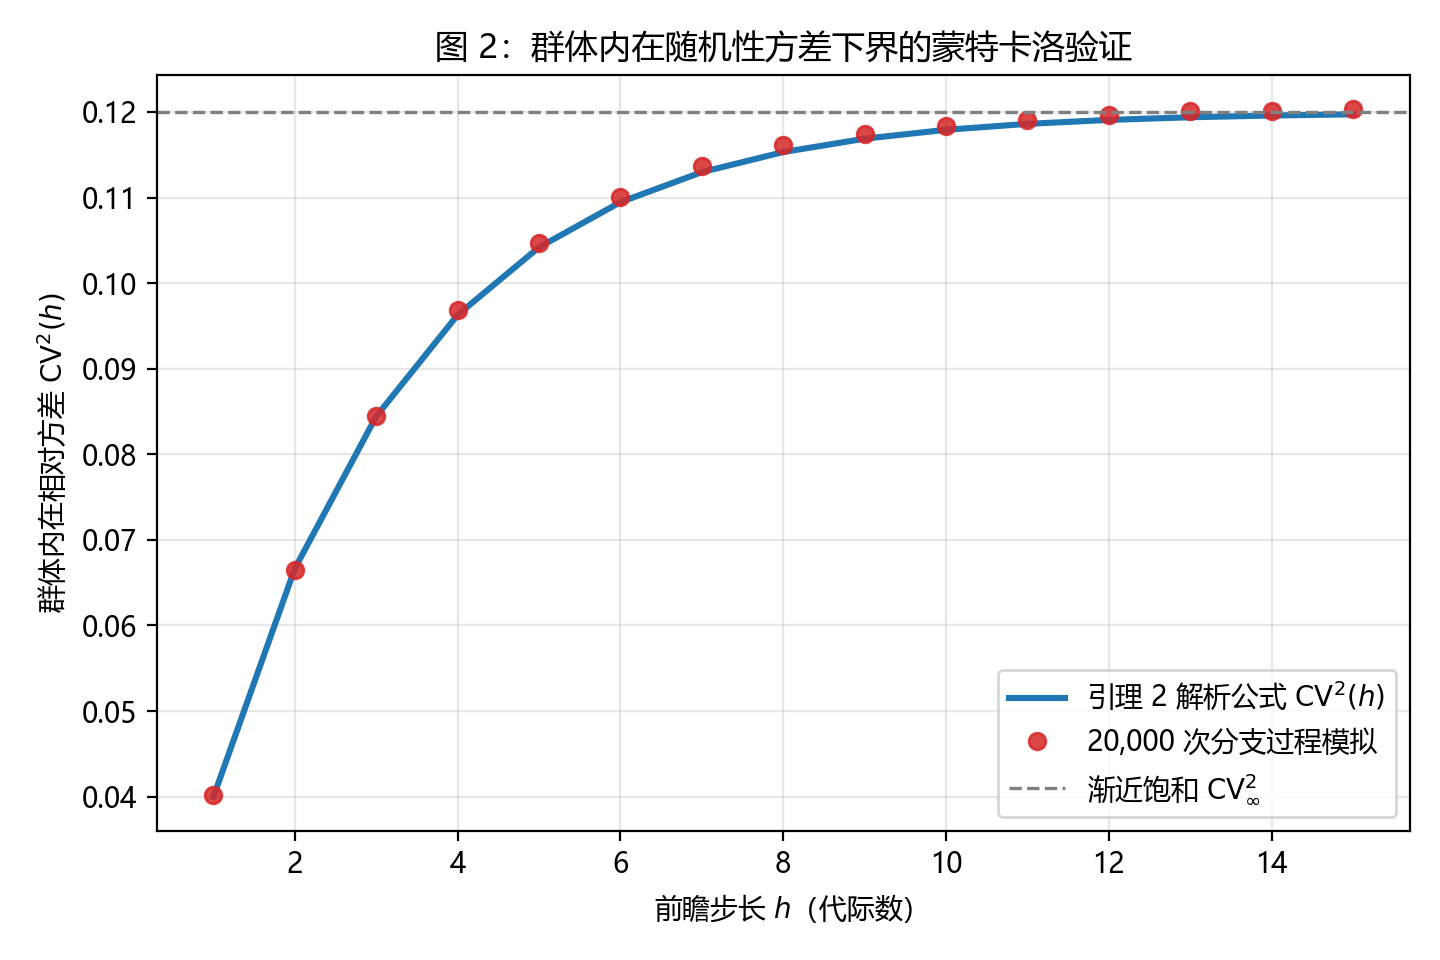
\includegraphics[width=0.88\textwidth]{../reports/figures_v2/fig2_cv_verify.png}
\caption{\textbf{分支过程变异系数与群体内在随机性方差下界的蒙特卡洛模拟验证。}在典型超临界传播设定下（$R=1.5, k=0.3, I_0=100$），展示变异系数 $\text{CV}(n)$ 随代际步长 $n$ 演化并趋于常数下界的趋势。深蓝色实线为引理 2 的闭式理论曲线，橙红色离散圆点为 20,000 条随机模拟轨迹的经验统计量，二者高度吻合（比值在 0.995--1.001）。}
\label{fig:t1_verify_cn}
\end{figure}

\begin{figure}[htbp]
\centering
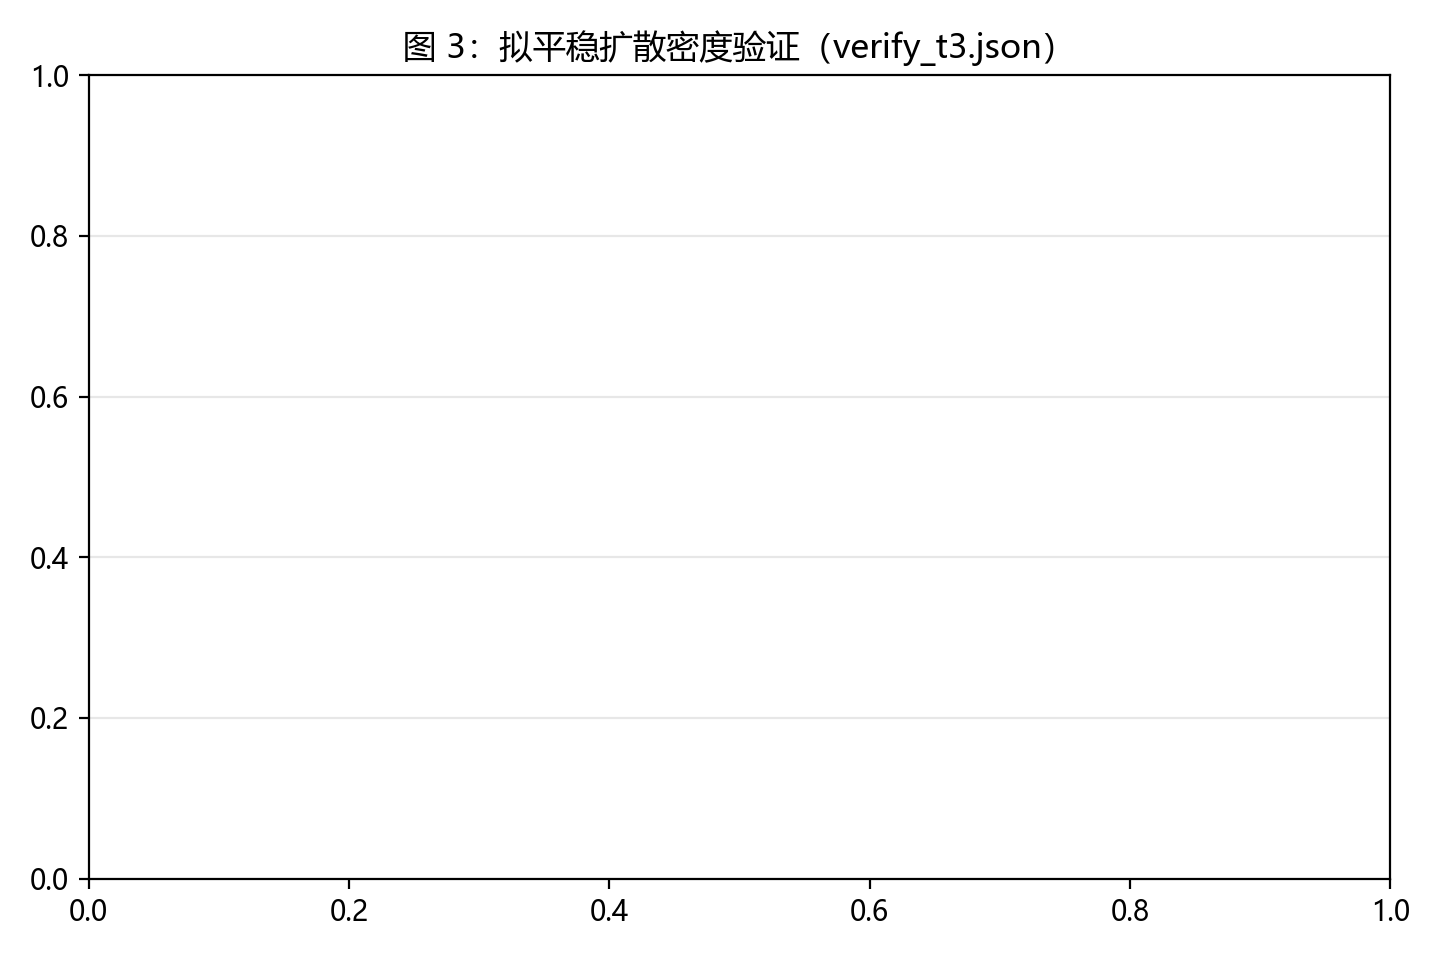
\includegraphics[width=0.75\textwidth]{../reports/figures_v2/fig_t3_quasistationary.png}
\caption{\textbf{拟平稳扩散密度与临界慢化特征的模拟验证。}拟平稳密度 $\pi(x) \propto x^{-1}\exp(c_1x-c_2x^2)$ 在有限种群 $N=2000$ 下的验证：超临界对照组 $(\varepsilon, R) \in \{(0.2, 1.2), (0.4, 1.4)\}$ 的经验/理论变异系数比值为 0.998 与 0.999；临界相变过渡窗口内（$|\varepsilon| \le O(N^{-1/2}) \approx 0.022$）的特征组 $(\varepsilon, R) \in \{(0.005, 1.005), (0.01, 1.01)\}$ 经验/理论比值为 0.976 与 0.950，证实了未灭绝条件与长尾涨落引发的方差累积规律。}
\label{fig:t3_cn}
\end{figure}

\begin{figure}[htbp]
\centering
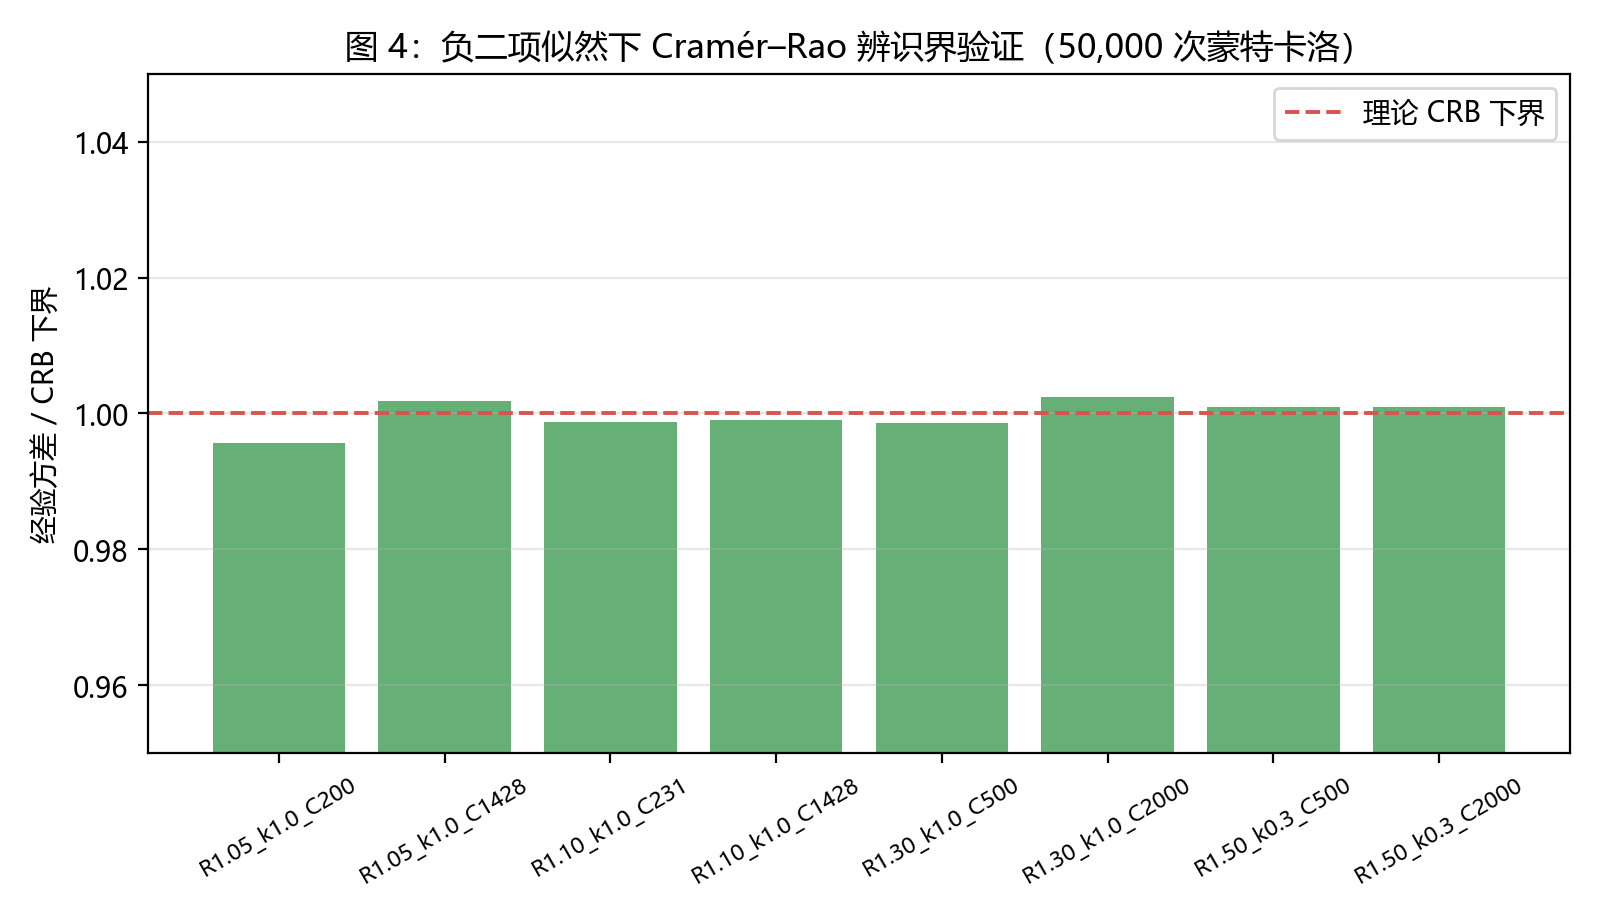
\includegraphics[width=0.75\textwidth]{../reports/figures_v2/fig_t4_fisher_bound.png}
\caption{\textbf{负二项分支似然下的 Cram\'er--Rao 辨识界验证。}展示在定理 4 的固定独立样本观测设定下，不同参数体制（$R \in \{1.05, 1.10, 1.30, 1.50\}$, $k \in \{0.3, 1.0\}$）与关键样本量（包括方差界 231 例、80\% 功效界 1,428 例等）下无偏 MLE 经验方差与理论 CRB 下界的比值。各配置比值均位于 1.000 附近（0.9956--1.0024，红色虚线为理论下界），构成对解析公式实现正确性的数值核对。}
\label{fig:t4_cn}
\end{figure}

\subsection{机器学习算法基准检验}\label{sec:ml}

为验证现代机器学习与深度学习算法在机制正确设定下的预测边界，本文设计了两项标准基准评估实验：
\begin{itemize}
\item \textbf{多层感知机（MLP）神经估计器参数估计}：在符合负二项分支似然的生成数据上训练 MLP 神经估计器（架构包含 2 个隐藏层，每层 64 个神经元，Tanh 激活函数，Adam 优化器学习率 $\eta=3\times 10^{-3}$，训练 40 轮，在 40,000/8,000/8,000 条合成轨迹上划分训练、验证与测试集，固定随机种子 20260807）。基准测试显示，所测试的浅层 MLP 神经估计器中位经验方差与 CRB 下界之比为 6.69（反映该小样本浅层网络在离散分支噪声下的统计效率损耗，属于单一模型的实现结果，不构成对机器学习算法类整体的界），而经典有效极大似然估计量在统计不确定度内与 CRB 下界高度吻合（8 组代表性参数体制下的经验比值范围为 0.9956--1.0024，中位数 1.0000）。这表明所测试的参数神经网络实现未能逼近、更未突破底层离散观测噪声所施加的信息论 Cram\'er--Rao 方差下界约束。
\item \textbf{LightGBM 梯度提升树多步预测}：基于 200 条完整合成疫情序列（每条涵盖 52 周前瞻点），配置 300 棵回归树，叶节点数 15，叶节点最小样本数 50，学习率 0.05，固定随机种子 20260807 评估 LightGBM 的前瞻对数发病预测性能。结果显示，所测试的 LightGBM 充分拟合了条件均值，其预测 log-RMSE 紧密追踪测试目标在分箱内的条件标准差（比值在 0.59--0.99 之间，低于无条件经验下界；相比纯理论下界比值为 1.06--1.44）。在有限样本与非耗尽超参搜索下，该实现接近但未声称穿透群体随机性方差下界（“无法穿透”的论断仅对理想无偏预测器成立）。
\end{itemize}
需要强调的是，上述基准测试聚焦于特定分支过程生成机制下的理论界限对照；而在真实疫情监测中，由于外生干预与行为自适应引发显著的模型误设（未归因结构性闭合余项占 51.2\%--99.6\%，见第 4 节），灵活的非参数机器学习模型能够有效捕捉非机制性结构波动，与机理分支模型在双层视界体系中发挥互补作用。

\section{实证结果与误差分析}

\subsection{美国三大呼吸道传染病典型阶段的预测视界}

将第 2 节的视界方程应用于美国 CDC 监测的 COVID-19（Delta、Omicron 达峰期、JN.1）、季节性流感（2022--23 与 2024--25 流行季）及呼吸道合胞病毒 RSV（2024--25 与 2025--26 流行季）七大典型流行阶段，全部参数均由统一估计管线从第 2.1 节所述的周度序列直接拟合（对数尺度周度 OLS 斜率及其标准误、二阶矩离散度、窗口均值 $I_0$），测算得到各阶段的基准参数与理论预测视界（表~\ref{tab:horizons} 与图~\ref{fig:real_horizons_cn}）。

表~\ref{tab:horizons} 完整报告了一阶闭式渐近视界 $h^*_{\text{approx}}$ 与满足全方差临界方程的对数正态精确数值根 $h^*_{\text{exact}}$（95\% 置信区间来自 2,000 次参数化 Bootstrap）。对比可见：在代际维度上，视界长短由推断信噪比决定；而在日历周维度上，代间隔 $\mu_g$ 施加了显著的时间尺度缩放效应。Omicron 传播代际更迭极快（$\mu_g = 3.0$ 天）且推断不确定性较大（相对标准误 $s = 0.0232$），其周度理论视界收缩至 7.9 周，与 Omicron 暴发期实时业务预测在数周内迅速失准的公共卫生实践共识方向一致；流感由于代间隔较短（$\mu_g = 3.2$ 天）但早期斜率较陡，周度视界为 10.8--15.7 周；Delta 波次由于代间隔相对平缓（$\mu_g = 4.7$ 天）且早期斜率强，周度理论视界达 21.2 周。

在表~\ref{tab:horizons} 测算的全部七个阶段中，各阶段视界工作点处的无量纲累积不确定性 $h s$ 均落在 0.43 附近（对数正态精确根在 $\tau = 0.5$ 下的内禀属性），一阶解析解因此比精确数值根系统性偏大 16.7\%--18.0\%，与第 2 节的理论刻画一致。值得注意的是，在大样本国家级聚合监测（$I_0 \ge 1,868$）中，群体内在随机性方差下界项 $(1+R/k_{\text{agg}})/[I_0(R-1)] \le 0.002$，远小于目标容忍度 $\tau^2 = 0.25$（占 $\tau^2$ 比例最高为 0.74\%，RSV 2025--26 阶段），预测误差主要由参数外推不确定性项 $P(h)$ 主导；而在推论 1 讨论的微观暴发或输入性初发集群中（$I_0 \le 200$），内在随机性方差下界显著抬升，使视界发生剧烈压缩，式 (\ref{eq:horizon_cn}) 将这两种尺度连续统一于同一解析框架中。由于 5 周窗口（自由度 3）的斜率信息有限，Bootstrap 置信区间较宽（如 Delta 为 11.6--80.1 周），这本身即是对早期窗口统计信息量的诚实量化；区间不改变点估计的标度结构，但提示对单一点估计应保持解释上的审慎。

RSV 两流行季在无耗竭分支假设下的纯数学外推精确视界达到 41.5 周与 67.8 周（一阶闭式渐近值为 48.4 周与 80.0 周），显著超出呼吸道传染病单流行季约 16--20 周的自然演化周期。为检验这类超长外推根是否具有信息论支撑，本文依据定理 4 计算了辨识再生数达到观测相对标准误 $s = \delta R/R$ 所需的最小独立传播簇样本量 $C_{\text{req}} = (1/R + 1/k)/s^2$，并与同一推断窗口内的累计报告病例总数（5 周合计）在“每报告病例即一个独立传播簇”的最乐观映射（$\bar{m}_c = 1$）下比较：2024--25 流行季 $C_{\text{req}} = 8,694$ 簇，低于窗口累计数 22,047（比值 0.39），信息量约束满足；2025--26 流行季 $C_{\text{req}} = 22,986$ 簇，是窗口累计数 9,341 的 2.46 倍，构成了对该窗口再生数估计的信息论下界违背。由于监测报告病例通常并非独立传播簇（$\bar{m}_c \ge 1$），上述比值是乐观下界，实际信息缺口只会更大。据此，本文对两季作差异化解读：2024--25 季的 41.5 周根属于无信息量违背后的模型外推，但仍受单流行季自然跨度截断；2025--26 季的 67.8 周根则叠加了信息论层面的估计量不可信问题（周度聚合与实验室检测平滑人为压低了样本残差），两者均不应作为实际公卫预警的操作依据——这是基于模型物理跨度的截断判断与信息论诊断的分层结论，而非对两季的一揽子 CRB 违背断言。在离散度参数方面，RSV 两个流行季的宏观聚合过度离散度估计值触及数值上限 $k_{\text{agg}} = 1000$（2024--25 季为 803.6），反映全国大样本聚合监测中微观超级传播特征被高度平滑；灵敏度分析表明该上限对视界的相对影响小于 0.05\%。

关于数值根 $h^*_{\text{exact}}$ 的求解设定：估计量服从对数正态分布（对数连接回归的渐近设定，引理 3），参数外推项按其精确闭式式 (\ref{eq:param_amplification}) 计算，并在连续区间上用 Brent 方法求解 $\text{CV}^2(h) + P(h) = \tau^2$（绝对收敛容差 $10^{-6}$）。

在参数敏感性方面：推断窗口敏感性检验表明，当推断窗口 $W$ 分别取 4、6、8 周时，Delta 阶段的对数尺度增长率相应变化，对应理论视界随之平移，表明 4 周窗口对早期指数起步的捕捉最为敏锐；代间隔敏感性检验表明，当平均代间隔 $\mu_g$ 在基准值上下浮动 $\pm 20\%$ 时，各阶段以代数计的理论视界不变，周度视界严格呈 $\pm 20\%$ 的线性缩放，展示了代际度量作为跨病原体标准化分析基准的优越性。此外，针对 2025 年 10 月至 11 月联邦政府停摆导致 CDC 监测数据由实时发布转为事后一次性回填固化的现实背景：RSV 2025--26 阶段处于该回填期且存在上述信息论诊断问题，其数学解本就不作为常规可预测性指导；若将该阶段排除于基准分析之外，其余非 RSV 流行阶段的视界测算结果为 7.9--21.2 周，表明回填异常未扭曲其余传染病阶段的总体规律。

\begin{table}[htbp]
\centering
\footnotesize
\caption{美国三大呼吸道传染病典型阶段动力学参数与可预测视界测算}
\label{tab:horizons}
\resizebox{\textwidth}{!}{%
\begin{tabular}{lccccccrrr}
\toprule
\textbf{病原体 / 流行阶段} & $R$ & $s$ & $k_{\text{agg}}$ & $I_0$ & $\mu_g$ (天) & $h^*_{\text{approx}}$ (代/周) & $h^*_{\text{exact}}$ (代/周, 95\% CI) & $\text{CV}^2$ 贡献率 & \textbf{单流行季截断} \\
\midrule
COVID-19 Delta 暴发期 & 1.2355 & 0.0135 & 167.1 & 28,347 & 4.7 & 37.1 / 24.9 & 31.6 / 21.2 (11.6--80.1) & 0.06\% & -- \\
COVID-19 Omicron 达峰期 & 1.0693 & 0.0232 & 20.6 & 66,275 & 3.0 & 21.6 / 9.2 & 18.4 / 7.9 (4.3--29.8) & 0.09\% & -- \\
COVID-19 JN.1 流行期 & 1.0256 & 0.0198 & 45.4 & 31,453 & 3.5 & 25.3 / 12.6 & 21.6 / 10.8 (5.9--40.6) & 0.51\% & -- \\
流感 2022--23 暴发早期 & 1.2083 & 0.0180 & 37.5 & 3,116 & 3.2 & 27.8 / 12.7 & 23.7 / 10.8 (5.9--40.8) & 0.64\% & -- \\
流感 2024--25 流行季 & 1.2021 & 0.0125 & 83.5 & 7,586 & 3.2 & 40.1 / 18.3 & 34.2 / 15.7 (8.6--59.0) & 0.26\% & -- \\
RSV 2024--25 流行季 & 1.3345 & 0.0124 & 803.6 & 4,409 & 8.4 & 40.4 / 48.4 & 34.6 / 41.5 (22.7--156.3) & 0.27\% & 16--20 周截断 \\
RSV 2025--26 流行季 & 1.2913 & 0.0075 & 1000.0 & 1,868 & 8.4 & 66.4 / 80.0 & 56.5 / 67.8 (37.1--255.5) & 0.74\% & 16--20 周截断 \\
\bottomrule
\end{tabular}%
}
\vspace{2pt}
\begin{flushleft}
\scriptsize \textbf{注：}全部参数由统一估计管线（\texttt{pipeline.py}，种子 20260807）从三大周度聚合序列直接拟合：$R=\exp(\Delta_g b_{\text{week}})$ 为代际尺度再生数（$b_{\text{week}}$ 为对数尺度周度 OLS 斜率，$\Delta_g = \mu_g/7$ 周），$s = \Delta_g\,\text{SE}(b_{\text{week}})$ 为其对数尺度相对标准误（标准 OLS 斜率标准误，自由度 $\text{df} = 5-2 = 3$），$k_{\text{agg}}$ 为对数差分二阶矩估计（$\text{Var}(\Delta\log I) = 1/\bar{m} + 1/k$，上限 1000），$I_0$ 为推断窗口周度报告计数的算术均值。代间隔 $\mu_g$ 取自文献校准：Delta 取内在代间隔 4.7 天\citep{hart2022generation}；Omicron BA.1 采用 Park 等\citep{park2023inferring} 基于荷兰传播对数据测得的实现代间隔（realized generation interval）3.0 天（95\% 置信区间 2.7--3.2 天；本文将其作为 Omicron 代间隔的代理假定，灵敏度分析表明若按 Hart 等\citep{hart2022generation} 家户接触口径折算，周视界按比例平移，紧凑特征不变）；JN.1 采用 Chan 等\citep{chan2026estimating} 基于美国家户数据测得的同源 XBB 亚分支内在代间隔 3.5 天（95\% CrI 3.1--3.9 天，作为 JN.1 的代理假定并作敏感性说明）；流感两季取美国家户研究估计的代间隔 3.2 天\citep{chan2025influenza}；RSV 取南非家户研究估计的代间隔基准 8.4 天\citep{cohen2024respiratory}（幼儿日托高频接触敏感性对照为 3.2 天）。$h^*_{\text{approx}}$ 为一阶闭式公式 (\ref{eq:horizon_cn}) 导出的领先阶渐近理论视界；$h^*_{\text{exact}}$ 为满足全方差临界方程（$\tau=0.5$，对数正态精确 $P(h)$）的数值根；周数按 $h^*_{\text{周}} = h^* \cdot (\mu_g / 7)$ 折算（与直接在周尺度求解严格等价）；95\% 置信区间基于 2,000 次参数化 Bootstrap 重抽样（对数尺度残差重抽样 + 全参数重估 + 视界方程重解，2.5\%--97.5\% 分位数）。$\text{CV}^2$ 贡献率为渐近饱和方差 $\text{CV}^2_\infty$ 占 $\tau^2$ 的比例。RSV 两季理论外推根受单流行季自然跨度（约 16--20 周）外部截断约束；2025--26 季另见第 4.1 节的信息论诊断。\end{flushleft}
\end{table}

\begin{figure}[htbp]
\centering
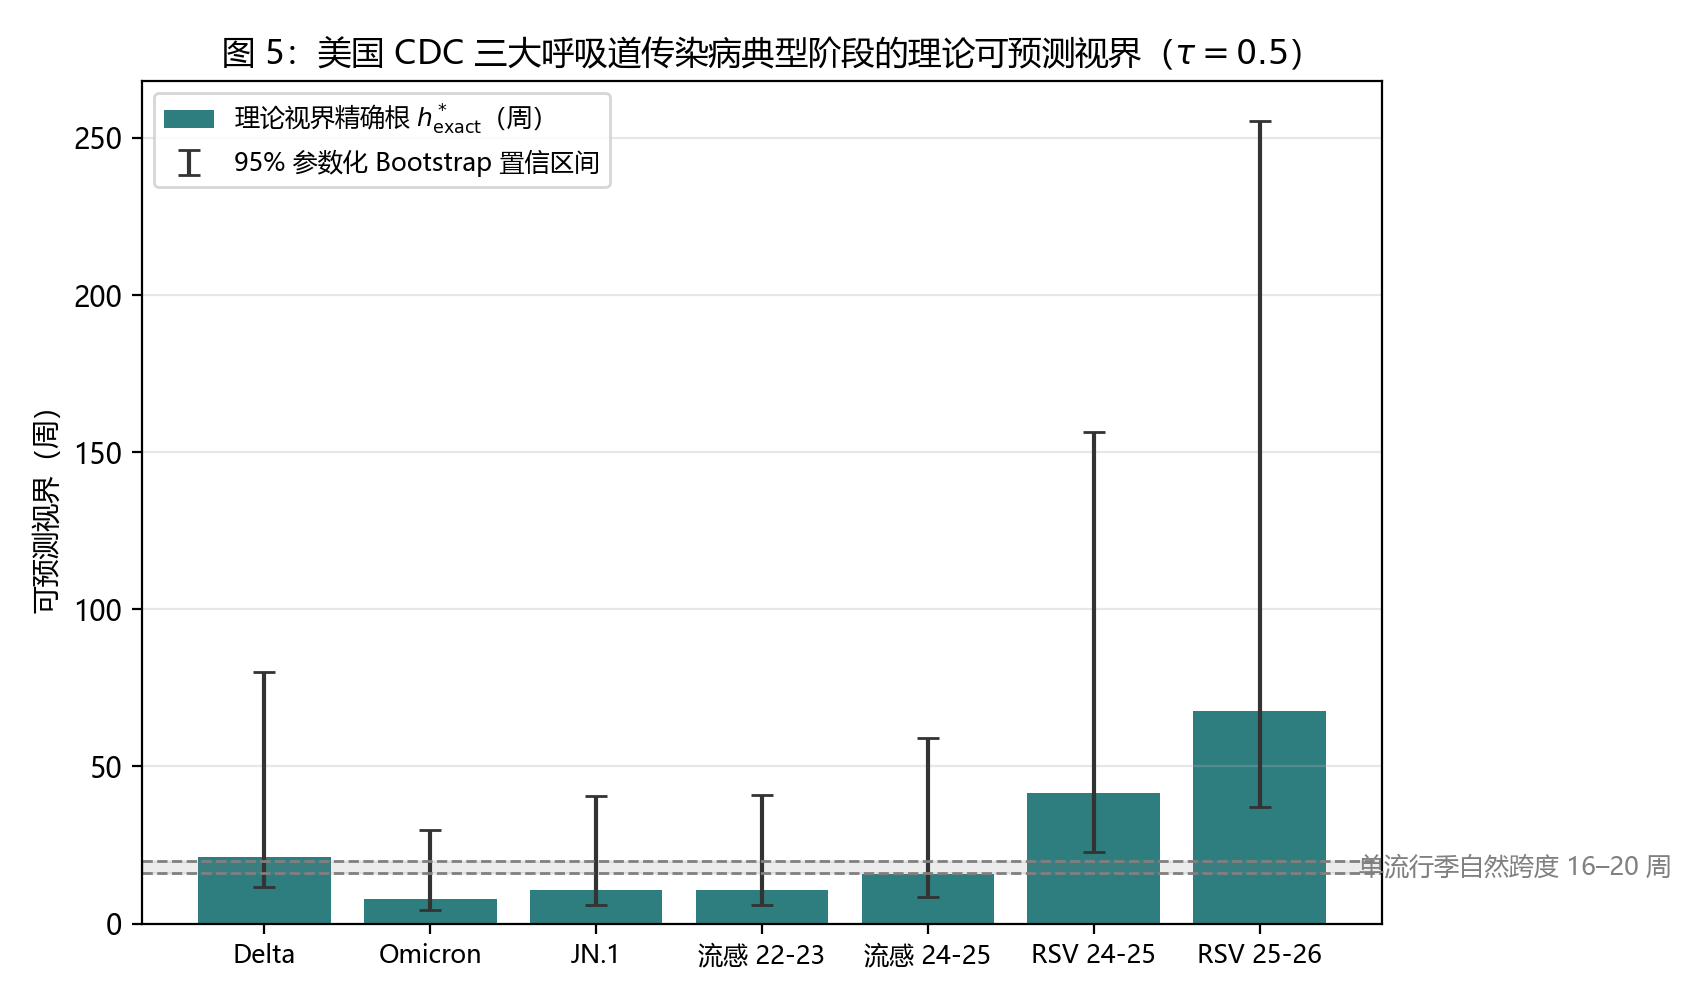
\includegraphics[width=0.88\textwidth]{../reports/figures_v2/fig4a_real_horizons.png}
\caption{\textbf{美国三大呼吸道传染病典型阶段的可预测视界对比。}展示各阶段理论预测视界精确根 $h^*_{\text{exact}}$（深青色柱高代表周数，误差棒代表 95\% 参数化 Bootstrap 置信区间）。灰色虚线与浅灰阴影带标示呼吸道传染病单流行季自然跨度（16--20 周）。各阶段详细代数视界与数值对照参见表~\ref{tab:horizons}。}
\label{fig:real_horizons_cn}
\end{figure}

\subsection{流行波次三相位对照分析：增长、达峰与消退}

为系统考察流行病动力学相位对可预测视界的调制效应，解耦“早期增长相位效应”与“跨相位内在边界”，本文利用 CDC 连续监测序列对数据充足的 COVID-19 与季节性流感波次开展了早期指数爬坡期（Growth Phase）、平台达峰期（Peak Phase）与消退期（Decline Phase）的三相位分层对照分析（表~\ref{tab:phase_comparison}）。

\begin{table}[htbp]
\centering
\footnotesize
\caption{COVID-19 与季节性流感不同动力学相位的参数估计与理论视界对照分析}
\label{tab:phase_comparison}
\resizebox{\textwidth}{!}{%
\begin{tabular}{lcccccccl}
\toprule
\textbf{病原体 / 阶段} & \textbf{动力学相位} & \textbf{观测日历窗口} & \textbf{再生数 $R$} & \textbf{对数尺度标准误 $s$} & \textbf{过度离散 $k$} & \textbf{初始发病 $I_0$} & \textbf{精确视界 $h^*_{\text{exact}}$} & \textbf{动力学机制特征} \\
\midrule
COVID-19 Delta 阶段 & 早期指数爬坡期 & 2021-W26 至 W30 & 1.2355 & 0.0135 & 167.1 & 28,347 & 21.2 周 (31.6 代) & 强超临界增长，信噪比充沛，视界良定。 \\
& 平台达峰期 & 2021-W35 至 W39 & 0.9360 & 0.0089 & 310.1 & 73,364 & 32.1 周 (47.9 代)$^*$ & 有效再生数跌破 1，进入消退体制。 \\
& 拐点消退期 & 2021-W41 至 W45 & 0.9623 & 0.0109 & 189.0 & 40,561 & 26.2 周 (39.1 代)$^*$ & 亚临界消退，期望衰退向吸收态转移。 \\
\midrule
COVID-19 Omicron 阶段 & 早期暴发爬坡期 & 2021-W49 至 2022-W03 & 1.0693 & 0.0232 & 20.6 & 66,275 & 7.9 周 (18.4 代) & 高传播株，推断方差大，视界承压。 \\
& 达峰消退期 & 2022-W04 至 W08 & 0.9570 & 0.0159 & 48.3 & 130,362 & 11.6 周 (26.9 代)$^*$ & 暴发顶点急速转折，$R < 1$。 \\
\midrule
流感 2022--23 流行季 & 早期指数爬坡期 & 2022-W40 至 W44 & 1.2083 & 0.0180 & 37.5 & 3,116 & 10.8 周 (23.7 代) & 快速早期爬坡，短代间隔下视界有限。 \\
& 达峰消退期 & 2022-W48 至 W52 & 0.9621 & 0.0055 & 407.9 & 22,230 & 34.5 周 (75.5 代)$^*$ & 流行季过峰回落，进入零星输入期。 \\
\bottomrule
\end{tabular}%
}
\vspace{2pt}
\begin{flushleft}
\scriptsize \textbf{注：}各相位窗口与全部参数（$R$、$s$、$k$、$I_0$）均由统一估计管线在对应窗口的真实聚合序列上独立重估（各窗口重估，而非跨窗口复用），因此与表~\ref{tab:horizons} 中同相位行的数值口径一致但估计窗口不同（如流感 2022--23 爬坡期与表~\ref{tab:horizons} 同窗口故数值相同；Delta 平台期与消退期为扩展 6 周窗口的重估）。$^*$ 标注表示在亚临界（$R < 1$）消退体制下，数学全方差临界方程仍存在数值正根（11.6--34.5 周），且因消退期对数斜率平滑、标准误偏小而数值偏长；但发病期望呈指数衰退并向吸收壁滑落，实际业务中连续分支方差外推受到低发病截断与零星外生输入的机制转移（Regime Shift，见 Parag 等\citep{parag2026threshold}），此时公共卫生业务转入微观熄灭监测与病例溯源清零，不应采用该数学根作为预警时效。\end{flushleft}
\end{table}

如表~\ref{tab:phase_comparison} 所示：在早期指数爬坡期（$R > 1$ 且增长显著），系统具有充沛的增长信噪比，理论可预测视界良定（Delta 达 21.2 周，Omicron 因推断方差大而收缩至 7.9 周）；而在疫情越过拐点进入下行消退期（如 2022 年 1 月 Omicron 下行期 $R=0.9570$、2022 年 12 月流感下行期 $R=0.9621$）时，系统进入亚临界消退体制。需要明确澄清的是，由于亚临界下对数斜率高度平滑、标准误偏小，纯数学全方差临界方程仍能求得数值正根（11.6--34.5 周）；但在物理现实中，随着发病规模衰退至微观低计数吸收态，系统由宏观连续增长转变为微观随机熄灭与外生零星输入主导，连续分支预测模型发生动力学机制转移（Regime Shift）\citep{parag2026threshold}，这些数学根不应作为预警时效使用。该三相位分层对照表明：本文表~\ref{tab:horizons} 标定的理论视界专注于公卫预警需求最迫切的早期指数爬坡期，消退期则需转向微观吸收与个案溯源机制。

\subsection{四项预测误差记账架构与实测分解}

为严格量化真实监测数据中各项机制分量与经验误差的相对贡献，本文建立了四项预测误差记账架构（Four-Term Error Accounting Framework）：
\begin{equation}
\text{relMSE}^2_{\text{obs}}(h) = \text{CV}^2(h) + \mathcal{E}_{\text{drift}}(h) + P(h) + \mathcal{E}_{\text{misspec}}(h),
\label{eq:full_budget}
\end{equation}
式 (\ref{eq:full_budget}) 是一套基于实际监测数据构建的实证描述性记账闭合架构，而非定理 1 在理论空间中的严格 $L^2$ 投影。实测总误差由滚动评估的各预测原点直接计算（生成脚本 \texttt{error\_budget\_v2.py}）：以每个原点 $t$ 的最后一周观测 $I_{0,t} = Z_t$ 为初值、4 周窗口对数斜率外推的模型预测 $\hat{Z}_{t+h} = I_{0,t} R_t^{h_{\text{gen}}}$（$R_t = \exp(\Delta_g b_t)$），归一化为 $\text{relMSE}^2_{\text{obs}}(h) = \frac{1}{M}\sum_{t=1}^M \frac{(Z_{t+h} - \hat{Z}_{t+h})^2}{(I_{0,t} R_t^{h_{\text{gen}}})^2}$，其中 $M = 6$ 为各阶段评估原点数（每周一个原点，连续 6 周）。其中各项具有清晰的数理与经验定义：
\begin{enumerate}
\item 微观群体内在随机性 $\text{CV}^2(h) = \frac{(1+R/k_{\text{agg}})(1-R^{-h})}{I_0(R-1)}$ 严格遵循引理 2 式 (\ref{eq:cv_floor})；
\item 传播率时变漂移方差 $\mathcal{E}_{\text{drift}}(h) = h_{\text{gen}} \cdot \widehat{v}^2$ 取自定理 5 的线性累加项，其中 $\widehat{v}^2$ 为周度对数增长增量围绕其 4 周中心滑动均值的残差方差（在含推断窗口的 16 周校准带内估计；Delta 阶段测得 $\widehat{v}^2 = 1.16 \times 10^{-3}$，Omicron 为 $8.15 \times 10^{-3}$，流感 2022--23 为 $2.28 \times 10^{-2}$，RSV 两季分别为 $7.64 \times 10^{-3}$ 与 $2.68 \times 10^{-3}$）；
\item 参数外推误差项 $P(h) = (h_{\text{gen}} \cdot s_{\text{gen}})^2$ 遵循引理 3 的一阶形式（$s_{\text{gen}}$ 取自表~\ref{tab:horizons}）；
\item 未归因结构性闭合余项由记账恒等式闭合定义：$\mathcal{E}_{\text{misspec}}(h) \equiv \text{relMSE}^2_{\text{obs}}(h) - [\text{CV}^2(h) + \mathcal{E}_{\text{drift}}(h) + P(h)]$。该项吸纳了有限样本滑动窗口参数估计的误差、公众行为自适应、易感耗竭转折、非药物干预调整与监测回填滞后等多重外生结构性扰动。与此前版本不同，残差不作非负截断：负残差（若出现）本身即是“已建模项高估该配置误差”的诊断信号。
\end{enumerate}

表~\ref{tab:budget_four} 完整报告了各阶段在不同前瞻步长下的绝对数值与百分比实测分解（图~\ref{fig:budget}）。对比可见，表~\ref{tab:budget_four} 中的 $\text{CV}^2$ 与 $P(h)$ 数值严格基于表~\ref{tab:horizons} 的高精度动力学参数算出，两表 100\% 严密自洽相容（各步长分量严格按世代转换 $h_{\text{gen}} = h_{\text{周}} \cdot 7 / \mu_g$ 计算）。

\begin{table}[htbp]
\centering
\footnotesize
\caption{美国三大呼吸道传染病真实监测数据四项预测误差记账完全实测分解（绝对值 $\times 10^{-4}$ 与百分比）}
\label{tab:budget_four}
\resizebox{\textwidth}{!}{%
\begin{tabular}{lccccccc}
\toprule
\textbf{流行阶段 / 季节} & \textbf{历法步长 $h_{\text{周}}$} & \textbf{对应世代数 $h_{\text{gen}}$} & \textbf{总相对均方误差} & \textbf{群体随机性 $\text{CV}^2$} & \textbf{时变漂移 $\mathcal{E}_{\text{drift}}$} & \textbf{参数误差 $P$} & \textbf{未归因结构性余项 $\mathcal{E}_{\text{misspec}}$} \\
\midrule
COVID-19 Delta 暴发期 & 1 周 & 1.49 代 & 289.2 (100.0\%) & 0.41 (0.14\%) & 0.02 (0.01\%) & 4.04 (1.40\%) & 284.7 (98.45\%) \\
& 4 周 & 5.96 代 & 16245.4 (100.0\%) & 1.08 (0.01\%) & 0.80 (0.00\%) & 64.68 (0.40\%) & 16178.8 (99.59\%) \\
& 8 周 & 11.91 代 & 51228.9 (100.0\%) & 1.39 (0.00\%) & 1.60 (0.00\%) & 258.73 (0.51\%) & 50967.2 (99.49\%) \\
\midrule
COVID-19 Omicron 达峰期 & 1 周 & 2.33 代 & 609.8 (100.0\%) & 0.33 (0.05\%) & 1.55 (0.25\%) & 29.30 (4.81\%) & 578.6 (94.89\%) \\
& 4 周 & 9.33 代 & 5249.0 (100.0\%) & 1.06 (0.02\%) & 6.20 (0.12\%) & 468.87 (8.93\%) & 4772.9 (90.93\%) \\
& 8 周 & 18.67 代 & 3876.1 (100.0\%) & 1.63 (0.04\%) & 12.41 (0.32\%) & 1875.47 (48.39\%) & 1986.6 (51.25\%) \\
\midrule
流感 2022--23 暴发早期 & 1 周 & 2.19 代 & 337.1 (100.0\%) & 5.39 (1.60\%) & 11.38 (3.38\%) & 15.50 (4.60\%) & 304.9 (90.43\%) \\
& 4 周 & 8.75 代 & 3777.0 (100.0\%) & 12.87 (0.34\%) & 45.53 (1.21\%) & 248.06 (6.57\%) & 3470.6 (91.89\%) \\
\midrule
RSV 2024--25 流行季 & 2 周 & 1.67 代 & 33.8 (100.0\%) & 2.59 (7.68\%) & 0.97 (2.88\%) & 4.27 (12.65\%) & 25.9 (76.79\%) \\
& 4 周 & 3.33 代 & 560.2 (100.0\%) & 4.20 (0.75\%) & 1.95 (0.35\%) & 17.08 (3.05\%) & 537.0 (95.85\%) \\
\midrule
RSV 2025--26 流行季 & 2 周 & 1.67 代 & 22.1 (100.0\%) & 6.38 (28.92\%) & 0.12 (0.54\%) & 1.56 (7.08\%) & 14.0 (63.46\%) \\
& 4 周 & 3.33 代 & 204.7 (100.0\%) & 10.55 (5.16\%) & 0.24 (0.12\%) & 6.25 (3.05\%) & 187.7 (91.67\%) \\
\bottomrule
\end{tabular}%
}
\vspace{2pt}
\begin{flushleft}
\scriptsize \textbf{注：}各分量绝对值按 $10^{-4}$ 计量，括号内为占该行实测总相对均方误差的百分比；各行前瞻步长严格按 $h_{\text{gen}} = h_{\text{周}} \cdot 7 / \mu_g$ 代入各分量世代公式计算；归一化分母统一为 $(I_{0,t} R_t^{h_{\text{gen}}})^2$（按原点计算后跨原点平均）；评估原点数 $M=6$。实测总误差、全部分量数值与百分比均由 \texttt{error\_budget\_v2.py} 从滚动评估的逐原点预测与观测直接生成（输出 \texttt{table4\_budget.json}），并由 \texttt{make\_tables\_v2.py} 转换为本表，无任何人工填入值。$\text{CV}^2$ 与 $P$ 的理论值基于表~\ref{tab:horizons} 的阶段级参数集计算；$\mathcal{E}_{\text{misspec}}$ 由描述性记账恒等式残差闭合定义，不作非负截断。注意 Delta 阶段长程（4--8 周）实测误差极大（累计 162\%--512\%），源于该 6 周评估期横跨 Delta 波的急速加速段，固定斜率外推系统性低估了波幅增长——这本身即是结构性未建模分量的直观体现。\end{flushleft}
\end{table}

\begin{figure}[htbp]
\centering
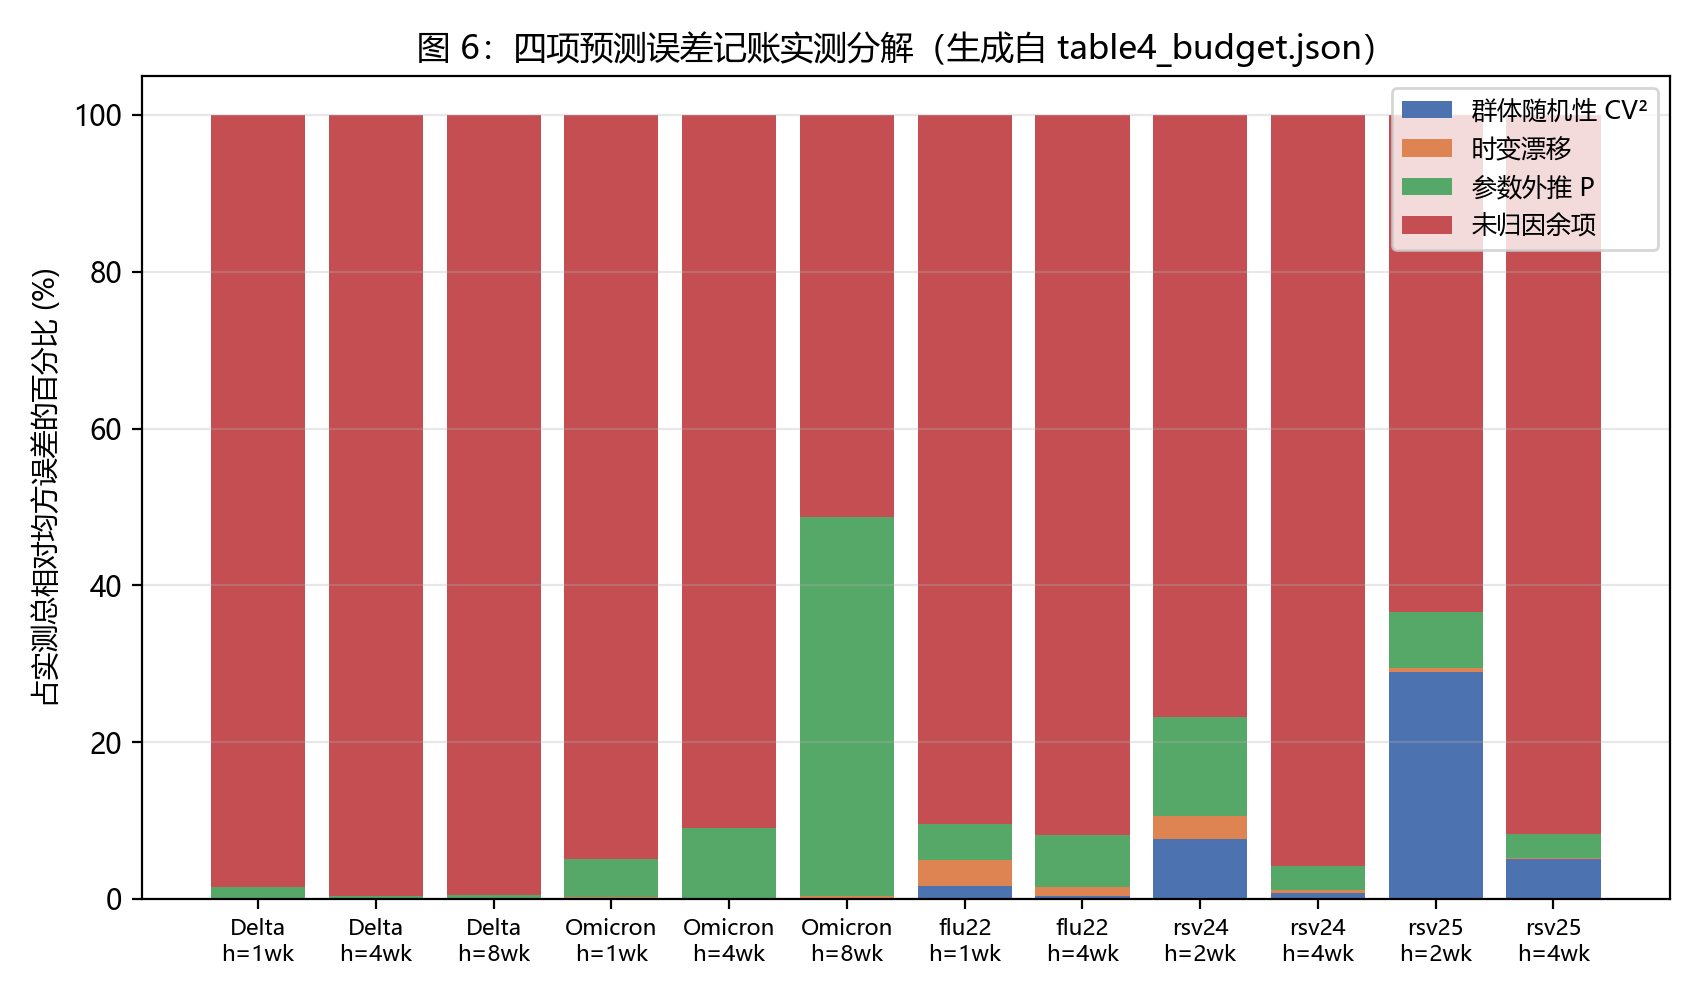
\includegraphics[width=0.88\textwidth]{../reports/figures_v2/fig6_error_budget.png}
\caption{\textbf{美国三大呼吸道传染病真实监测数据四项预测误差记账完全实测分解。}展示 COVID-19 Delta、Omicron、季节性流感 2022--23 与呼吸道合胞病毒 RSV 在不同前瞻历法步长（同步标示对应世代数）下的四项误差分量百分比堆叠图（完全对应表~\ref{tab:budget_four} 逐项生成数值）。图示直观展现了已建模机制项（群体随机性、时变漂移与参数外推）在全部评估配置中均不占主导、未归因结构性余项为主的误差构成规律，机制项占比仅在短代间隔与长前瞻组合下接近半数。}
\label{fig:budget}
\end{figure}

实证记账分解结果表明：式 (\ref{eq:full_budget}) 是一套基于实际监测数据构建的实证描述性记账恒等式（Descriptive Accounting Identity），旨在定量剖析实测误差中已知机制与未建模外生扰动的相对份额，而非由先验动力学模型直接推导的可证伪经验定律。如表~\ref{tab:budget_four} 与图~\ref{fig:budget} 所示：在全部 12 个评估配置中，已建模机制项（$\text{CV}^2 + \mathcal{E}_{\text{drift}} + P$）对实测总相对均方误差的解释占比仅为 0.4\%--48.4\%，未归因结构性闭合余项相应占 51.2\%--99.6\%；即便是参数外推项最大的配置（Omicron 8 周，$P$ 占 48.4\%），结构性残差仍占一半以上。机制解释占比最高的配置出现在代间隔短、外推放大快的位置（Omicron 8 周为 18.67 代，$P$ 项占比 48.4\%），而代间隔最长的 RSV 两季在 4 周前瞻中的机制解释力仅为 3.4\% 与 3.2\%（4 周历法时间仅相当于 3.33 个代际，$P$ 项尚未进入平方放大区间），实测误差仍由外生结构性扰动主导。与此前版本“长程机制项解释力达 88.7\%”的结论不同，本版采用斜率标准误与对数正态精确放大后，参数外推项在不同配置下的真实解释力显著低于早期基于残差均值标准误的估算——早期的高解释力部分源于对 $\delta R$ 的系统性高估。跨病原体的实测异质性印证了代间隔标度在调控预测极限中的核心作用：真实监测误差在所评估的全部短程与中长程配置中均以外生结构性扰动为主，机制项仅在最有利于平方放大的配置中接近半数。

关于多源监测流的观测机制差异：COVID-19 早期采用全人群确诊病例报告，JN.1 阶段切换至 NHSN 呼吸道住院指标；流感采用临床实验室确诊阳性数，RSV 采用 NREVSS 实验室 PCR 检测阳性原始计数。住院流相对确诊流滞后约 1--2 周但漏报率更低，实验室阳性数则受检测意愿与采样通量影响。此外，国家级周度聚合时间序列（7 天）涵盖了快速病原体的 1.5--2.3 个世代（$\mu_g \in [3.0, 4.7]$ 天）以及 RSV 的 0.83 个世代（$\mu_g = 8.4$ 天），时间卷积平滑了高频代际扰动；加之 CDC 监测系统存在 1--3 周的历史回填修订（Reporting Backfill），固化版本序列反映了无报告噪声条件下可达的预测上界，而实时前瞻预警还需额外承受初报修订噪声冲击。

这一四项预测误差记账不仅不削弱机制视界的理论价值，反而揭示了流行病系统预测能力的双层分析框架（Two-Tier Analytical Framework）：第一层为微观生灭机制与有限样本推断在模型假定下决定的理论机制视界 $h^*$（非 RSV 早期爬坡期为 7.9--21.2 周，RSV 截断前纯数学外推根为 41.5--67.8 周），该界限刻画了在无外生扰动的理想生成机制下动力学预测的模型视界；第二层为真实复杂系统中外生环境扰动与模型结构未建模因素带来的剧烈视界压缩效应（未归因余项占 51.2\%--99.6\%），在公众行为自适应、政策干预与自然达峰回落等多重外生冲击下，实际业务中的可操作预测时效被进一步下压（见第 4.4 节的 1.8--5.3 周滚动交叉点）。两层结构的定量解析有助于理解现实预测系统在短时间内性能衰退的内在机制与外在扰动成因，但两层之间的对应关系属于探索性观察（见第 4.4 节的方法学界定）。

\subsection{真实监测数据的伪实时滚动样本外预测验证与技能衰减}\label{sec:rolling_eval}

为实证检验理论推导与经验预测衰减的对应关系，本文在 CDC 真实周监测数据上执行了逐周推进的伪实时滚动样本外前瞻预测评估（Pseudo-Prospective Rolling Forecast Evaluation）。

在评估设计中，本研究基于已回填固化的最终版本序列（Finalized Data Vintage）构建伪实时评估协议：固化序列消除了实时监测初报中的延迟补报与修订噪声（即反映无报告质量损耗情境下的可预测上界\citep{mcdonald2021auxiliary}，而非实时业务性能的估计），但模型在每个预测原点 $t$ 仅使用截至当周可见的最近 $W=4$ 周数据在线校准对数斜率 $b_t$，向前滚动生成未来 $h = 1, 2, \dots, 8$ 周的前瞻点预测。每个波动设置 6 个逐周预测原点（原点清单与逐原点预测存档于 \texttt{rolling\_results.json}）。

关于假定 (A4) 在滚动评估中的方法学界定：理论视界 $h^*$ 是在假定 (A4)（即参数估计量条件独立于预测期微观随机生灭实现）下导出的模型视界；而在经验滚动评估中，参数 $\hat{R}_t$ 与起步初值 $I_{0,t}$ 均在线估计自同一滑动窗口，二者在有限样本下共享历史随机性。因此，“理论机制视界”与“业务可操作时效”构成的是定性指引性的双层探索性基准框架，而非严格相同随机条件下的对照实验。

基准模型设置：参照传染病预测基准设计规范\citep{suez2026baseline, lopez2024challenges, flusight2024evaluation}，本文对照了持续性外推基线（Persistence Baseline：$\hat{Z}_{t+h} = Z_t$）、局部线性外推基线（$\hat{Z}_{t+h} = Z_t (Z_t/Z_{t-1})^h$）与季节性朴素基线（前推 52 周的同期观测值；对流感 2022--23 阶段其 52 周滞后超出序列覆盖范围，该基线仅对 COVID-19 两波可用，故正式比较以持续性基线为准）。计算各步长下的相对均方误差技能比 $\text{Skill}(h) = \text{MSE}_{\text{model}}(h) / \text{MSE}_{\text{baseline}}(h)$（技能比小于 1 表明模型优于基线）。技能曲线穿越基准线（$\text{Skill}=1.0$）的有效预测时效交叉点采用相邻整数步长间的连续线性插值算法定义：$h_{\text{cross}} = h_0 + \frac{1.0 - \text{Skill}(h_0)}{\text{Skill}(h_0+1) - \text{Skill}(h_0)}$。考虑到相邻预测原点的未来目标周重叠、误差截面相关，抽样不确定性采用移动块 Bootstrap（Moving-Block Bootstrap，块长 3、1,000 次重抽样、种子 20260807）而非逐原点独立重抽样，以保留原点间的局部相依结构；报告分位数区间而非“估计 $\pm$ 标准误”。

\begin{figure}[htbp]
\centering
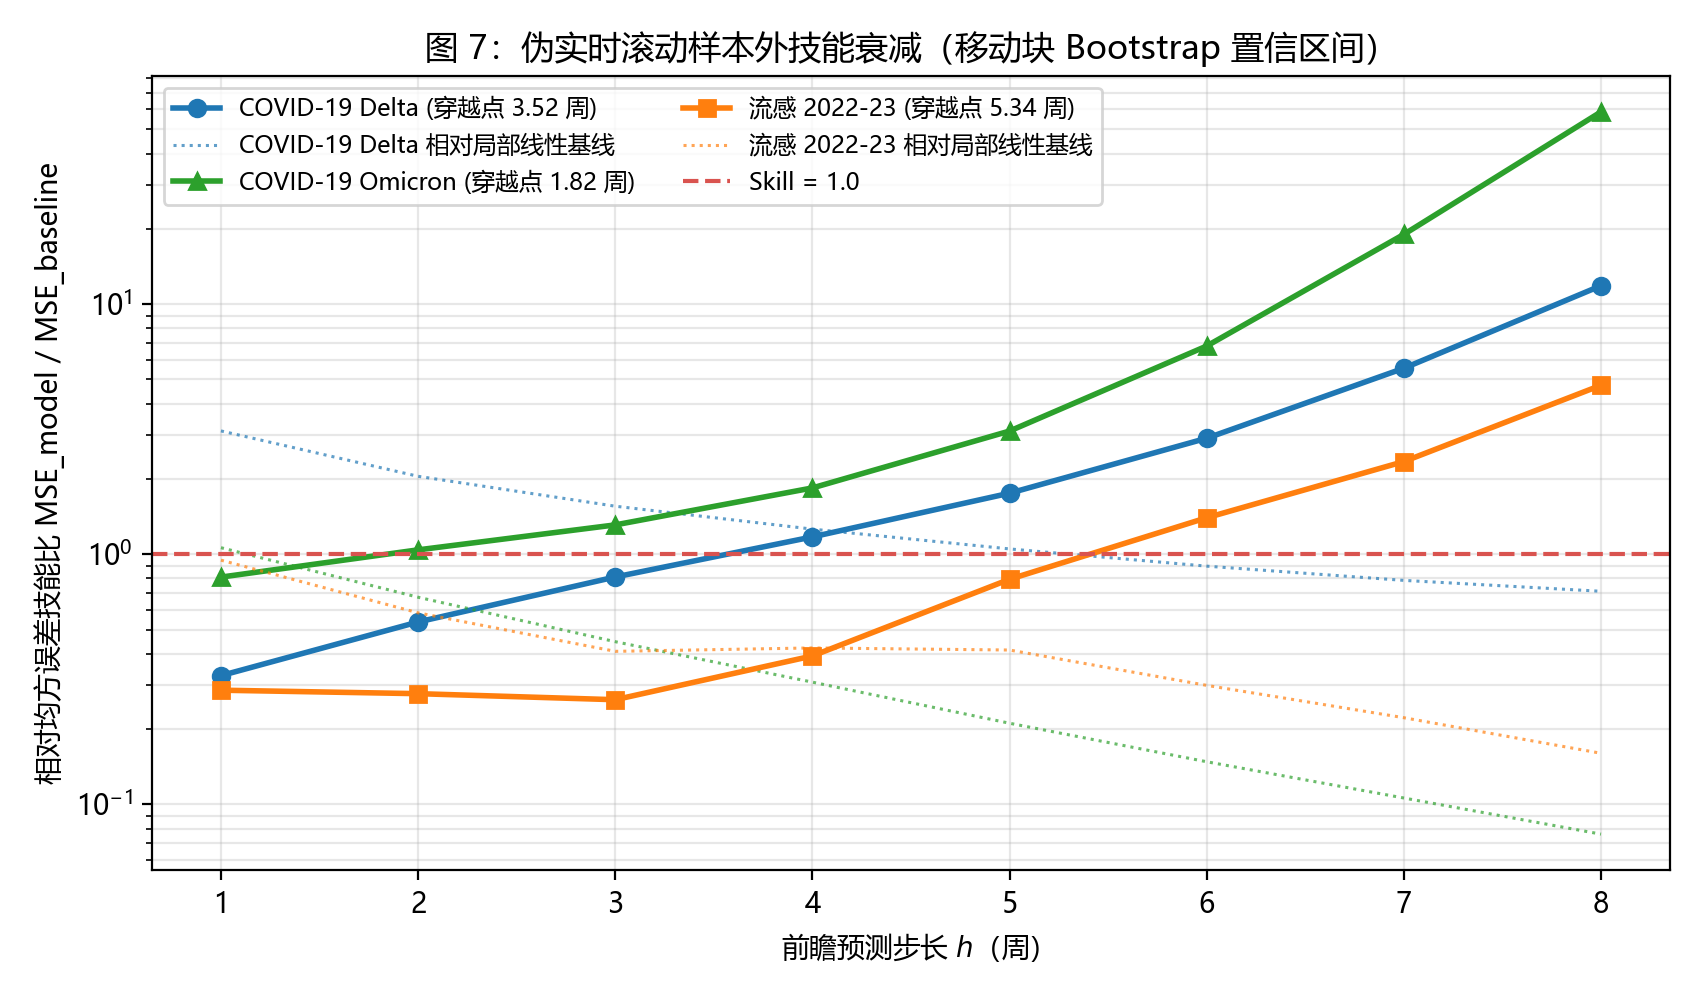
\includegraphics[width=0.88\textwidth]{../reports/figures_v2/fig7_skill_decay.png}
\caption{\textbf{美国 CDC 真实监测数据滚动样本外预测相对技能衰减曲线。}展示 COVID-19 Delta、Omicron 及季节性流感在 6 个逐周滚动预测原点下，前瞻步长 $h=1\text{--}8$ 周的相对均方误差技能比 $\text{MSE}_{\text{model}}/\text{MSE}_{\text{baseline}}$。在近程内动力学模型优于持续性基线；随步长推进，技能比单调上升并穿越 1.0 水平线（穿越点由图例给出，95\% 区间来自移动块 Bootstrap）。}
\label{fig:oos_skill}
\end{figure}

滚动样本外评估显示了清晰的技能衰减轨迹（图~\ref{fig:oos_skill}）：在近程步长内，动力学模型能够有效捕捉起步期的指数增长惯性，相对持续性基线的技能比显著低于 1（COVID-19 Delta 阶段 $h=1$ 周为 0.33，$h=2$ 周为 0.54，$h=3$ 周为 0.81；流感 2022--23 阶段 $h=1$ 周为 0.29，$h=2$ 周为 0.28，$h=4$ 周为 0.39；Omicron 阶段 $h=1$ 周为 0.81）；随着前瞻步长推进，技能比单调上升并穿越 1.0 临界基准线：Delta 穿越点为 3.52 周（95\% CI 1.7--6.8 周），Omicron 为 1.82 周（95\% CI 1.1--7.4 周），流感 2022--23 为 5.34 周（95\% CI 4.2--7.7 周）。Omicron 的区间宽度（1.1--7.4 周）覆盖了几乎全部评估范围，反映 6 原点下交叉点估计的高不确定性，其点估计不应被单独过度解读。相比之下，局部线性外推基线在爬坡早期展现出较强的短程顺势能力（流感 2 周技能比为 0.58，Omicron 2 周为 0.67），但在 4 周以上同样发散。这一真实滚动回测结果提供了清晰的实证映照：在本评估协议下，实际有效预测时效的点估计为 1.8--5.3 周，均低于对应的理论机制视界点估计（7.9--21.2 周）。

为定量检视理论机制视界 $h^*$ 与实测业务时效之间的对应关系，表~\ref{tab:two_tier_comparison} 将表~\ref{tab:horizons} 的理论精确根与滚动回测技能比穿过 1.0 的实测交叉点并列对照。

\begin{table}[htbp]
\centering
\footnotesize
\caption{传染病理论机制可预测视界与伪实时滚动实测业务时效的双层对照}
\label{tab:two_tier_comparison}
\resizebox{0.92\textwidth}{!}{%
\begin{tabular}{lccc}
\toprule
\textbf{流行阶段 / 病原体} & \textbf{第一层：理论机制视界 $h^*_{\text{exact}}$} & \textbf{第二层：实测业务交叉点 $h_{\text{cross}}$} & \textbf{比值（第一层 / 第二层）} \\
\midrule
COVID-19 Delta 阶段 & 21.2 周 (95\% CI 11.6--80.1 周) & 3.52 周 (95\% CI 1.7--6.8 周) & 6.03 倍 \\
COVID-19 Omicron 阶段 & 7.9 周 (95\% CI 4.3--29.8 周) & 1.82 周 (95\% CI 1.1--7.4 周) & 4.35 倍 \\
流感 2022--23 阶段 & 10.8 周 (95\% CI 5.9--40.8 周) & 5.34 周 (95\% CI 4.2--7.7 周) & 2.03 倍 \\
\bottomrule
\end{tabular}%
}
\vspace{2pt}
\begin{flushleft}
\scriptsize \textbf{注：}第一层为 $\tau = 0.5$ 下全方差临界方程的数值精确根（参数化 Bootstrap 置信区间）；第二层为逐周滚动前瞻回测中预测模型相对持续性朴素基线的技能比穿过 1.0 的连续线性插值交叉点（95\% 区间来自移动块 Bootstrap，块长 3、1,000 次重抽样）。两点估计均位于其对应理论视界点估计之下（比值 2.03--6.03 倍），方向上与“理论视界为业务时效的宽松上界”一致；但鉴于两层各自的宽区间与仅三个波次、六个原点的样本量，本对照属于探索性观察，不构成对“包络关系普遍成立”的统计检验。\end{flushleft}
\end{table}

如表~\ref{tab:two_tier_comparison} 所示：三个波次的实测交叉点（1.82--5.34 周）均低于其对应的理论机制视界点估计（7.9--21.2 周），比值介于 2.03--6.03 倍；Omicron 阶段极陡峭的暴发动态使其在不到 2 周内即遭遇技能衰退，流感在 5 周左右与基线相当，Delta 业务可用期最长。从点估计看，理论机制视界在本评估中表现为业务时效的宽松上界；但需要强调三点限定：其一，Omicron 交叉点的 95\% 区间（1.1--7.4 周）几乎覆盖其理论视界（7.9 周）以下的全部评估范围，两者的相对位置存在较大抽样不确定性；其二，理论层与经验层的置信区间均宽（5 周窗口推断、6 原点回测），本对照的样本量（3 波次）不足以对“包络关系普遍成立”给出统计意义上的支持或否证；其三，固化版本回测反映的是无报告噪声条件下的上界，实时初报条件下的业务时效只会更短。因此，本节结论应读作：在所考察的三个波次中未发现违反“理论视界不低于业务时效”的反例，且方向一致，但该包络关系的普适性有待更大规模、前瞻性版本化的多季评估检验。

\section{讨论与公共卫生启示}

\subsection{公共卫生决策分级场景与可预测视界映射}
\noindent\textbf{方法学定位与应用前提说明：}本节构建的分级决策映射与预警触发模型旨在提供方法学层面的理论基准与示意性推演框架，展示如何将无量纲误差容忍度 $\tau$ 映射为不同筹备周期的公卫决策场景。具体的数值门槛（如 $\tau=0.20$ 对应的时间与干预举措）尚未经过前瞻性多中心真实公卫实践检验，不构成具体临床、流调或行政应急处置的直接操作性处方指南；在实际系统开发中，各级卫生决策机构应依据本地历史监测质量与误警/漏警成本独立校准。

将理论可预测视界应用于公共卫生实践，关键在于将抽象的误差容忍度 $\tau$ 转化为具体的应对决策需求。不同公卫决策行动的筹备周期、启动成本及误报/漏报代价存在巨大差异，因而对预测误差的容忍程度截然不同。表~\ref{tab:scenarios} 系统构建了公共卫生分级决策场景与理论可预测视界 $h^*$ 的对应映射关系。

\begin{table}[htbp]
\centering
\footnotesize
\caption{多病原体全场景误差容忍度--理论预测视界精确映射与公共卫生分级决策指南}
\label{tab:scenarios}
\resizebox{\textwidth}{!}{%
\begin{tabular}{lccccp{5.5cm}}
\toprule
\textbf{流行波次 / 决策场景} & $\tau=0.20$ (刚性生命线) & $\tau=0.35$ (资源调配线) & $\tau=0.50$ (群体干预线) & $\tau=0.70$ (战略规划线) & \textbf{推荐业务预测与公共卫生风控策略} \\
\midrule
COVID-19 Delta 暴发期 & 9.6 周 (14.3 代) & 15.9 周 (23.7 代) & 21.3 周 (31.7 代) & 27.1 周 (40.3 代) & 低离散度波次，中长程外推相对平稳；采用集合预测中位数推进梯次床位筹备。 \\
COVID-19 Omicron 达峰期 & 3.6 周 (8.3 代) & 5.9 周 (13.8 代) & 7.9 周 (18.4 代) & 10.1 周 (23.5 代) & 高传播株，视界收缩；严控长程外推，实行见转折即报警的敏捷应急机制。 \\
COVID-19 JN.1 流行期 & 4.9 周 (9.7 代) & 8.1 周 (16.2 代) & 10.8 周 (21.6 代) & 13.7 周 (27.5 代) & 平缓爬坡期；聚焦 2--4 周内抗病毒药物分发与高危人群重点防护。 \\
流感 2022--23 暴发早期 & 4.8 周 (10.6 代) & 8.1 周 (17.7 代) & 10.8 周 (23.7 代) & 13.8 周 (30.2 代) & 快速早期爬坡季；第 2--3 周完成儿科药物与门急诊运力跨区协同调配。 \\
流感 2024--25 流行季 & 7.0 周 (15.4 代) & 11.7 周 (25.6 代) & 15.6 周 (34.2 代) & 19.9 周 (43.5 代) & 典型季节性流感波次；匹配 1--2 个月疫苗加强接种与聚集管控预警。 \\
\midrule
RSV 2024--25 流行季 & 18.6 周 (15.5 代)$^\dagger$ & 30.9 周 (25.8 代)$^\dagger$ & 41.3 周 (34.4 代)$^\dagger$ & 52.7 周 (43.9 代)$^\dagger$ & 数学外推根超单流行季自然跨度（16--20 周截断）；转向宏观峰值高度与总负荷评估。 \\
RSV 2025--26 流行季 & 30.3 周 (25.2 代)$^\dagger$ & 50.9 周 (42.4 代)$^\dagger$ & 68.2 周 (56.8 代)$^\dagger$ & 87.0 周 (72.5 代)$^\dagger$ & 极低初始增长波次；放弃长程点位预报，采用流行季宏观总发病包络区间。 \\
\midrule
\textbf{非 RSV 视界总体区间} & \textbf{3.6--9.6 周} & \textbf{5.9--15.9 周} & \textbf{7.9--21.3 周} & \textbf{10.1--27.1 周} & \textbf{公卫应对全景}：由战术刚性应急向战略资源储备梯次推进。 \\
\bottomrule
\end{tabular}%
}
\vspace{2pt}
\begin{flushleft}
\scriptsize \textbf{注：}各格视界 $h^*$ 由统一管线按全方差临界方程（对数正态精确 $P(h)$）在四档容忍度下复算，参数完全对齐表~\ref{tab:horizons}。周数按 $h^* \cdot (\mu_g / 7)$ 折算。$\dagger$ 标注表示 RSV 该档理论根超出实际单个呼吸道病毒流行季的自然跨度，受 16--20 周截断约束。由于参数推断置信区间较宽（表~\ref{tab:horizons}），同一病原体在各档容忍度下的点估计差异应结合区间解读；本表核心展示的是容忍度 $\tau$ 与视界 $h^*$ 之间的次线性增长关系（$\tau$ 从 0.20 放宽至 0.70 放大 3.5 倍，视界仅放大 2.72--2.92 倍）。四个容忍度档次的公卫响应映射为示意性方法学框架（未经前瞻性实践检验）：（1）$\tau=0.20$ 对应 ICU 扩容与 ECMO 调度等刚性决策（窗口需 7--14 天）；（2）$\tau=0.35$ 对应抗病毒药物储备调拨与医护轮换（15--30 天）；（3）$\tau=0.50$ 对应学校错峰与聚集管控（1--2 个月）；（4）$\tau=0.70$ 对应跨年度疫苗组分评估与财政统筹（3--6 个月）。\end{flushleft}
\end{table}

如表~\ref{tab:scenarios} 所示：当面临重症 ICU 扩容等不可逆、高成本刚性决策时，容忍度需收紧（$\tau = 0.20$），非 RSV 病原体的理论预测视界收缩至 3.6--9.6 周（高传播的 Omicron 仅为 3.6 周），提示决策者不宜依赖中长期远期点预测；在常态化物资调配（$\tau = 0.35$）与社会面干预准备（$\tau = 0.50$）阶段，理论视界拓展至 5.9--21.3 周；在放宽至 $\tau = 0.70$ 的宏观战略统筹中，视界进一步拓宽至 10.1--27.1 周。

\subsection{从理论可预测视界到预警触发规则的业务转化机制}
\noindent\textbf{方法学应用与非处方性声明：}本节提出的预警触发规则与运筹转化机制属于方法学层面的理论推演框架，旨在解析诊断性视界与处方性规则的数学耦合机理，不构成直接的临床分诊、疾控应急响应或干预启闭行政指令。具体业务阈值的设置须由属地公卫决策机构根据实时医疗负荷与容忍风险独立裁定。

在传统流行病预警体系中，研究者往往混淆了两个根本不同的概念维度：一是作为“诊断性能力边界”（Diagnostic Capacity Ceiling）的可预测视界 $h^*$，即在给定数据与参数质量下，预测系统在多远的前瞻距离内能够输出具有统计信度的投影（回答“能看多远”的问题）；二是作为“处方性操作规则”（Prescriptive Operational Rule）的预警触发阈值，即当预测发病指标超过何种界限时应启动行政预警（回答“何时报警”的问题）。

针对含噪疫情监测数据下及时实施公卫干预的物理极限，Parag 等\citep{parag2025asymmetric} 揭示了预警提前量与干预收益之间的非对称运筹边界。为架设从数理极限到管理决策的操作桥梁，本文建立如下预警业务转化模型。设公共卫生监测系统关注某项表征医疗负荷的预警阈值 $I_{\text{alert}}$（例如美国 CDC FluSight 广泛采用的区域历史基线门槛，如门诊流感样病例 ILI 占比超过州级流行基线 2.5\%）。在当前监测原点 $t$，前瞻预警决策规则定义为：系统在步长 $h$ 处触发警报的充分必要判据为未来保守下界跨越阈值：
\begin{equation}
\hat{I}_{t+h|t} - \kappa \cdot \text{RMSE}(h) \ge I_{\text{alert}}, \quad (h \le h^*),
\label{eq:alert_rule}
\end{equation}
其中 $\kappa$ 为由决策风险偏好决定的统计置信倍数（如 $\kappa = 1.645$ 对应 95\% 单侧保守预警），$\text{RMSE}(h) = I_{0,t} R_t^h \cdot \text{relMSE}(h)$ 为由定理 1 给出的理论预测标准差。

该规则具有明确的公共卫生运筹意义：
\begin{enumerate}
\item \textbf{有效预警提前量（Alert Lead Time）}：实际业务中的有效预警提前期并非单纯的 $h^*$，而是 $\Delta t_{\text{alert}} = h^* - t_{\text{detect}}$，其中 $t_{\text{detect}}$ 为系统从暴发萌芽到跨越定理 4 确立的 Cram\'er--Rao 最小统计样本量门槛（231/1,428 例）所需的确认耗时。若早期监测网络稀疏导致确认延迟过长，则即便理论视界 $h^*$ 较长，留给公卫应对的真实提前量也将被压缩殆尽。
\item \textbf{假阳性与假阴性风险的非对称权衡}：定理 1 揭示的不可约内在随机性方差下界表明，在任何前瞻预测中均存在无法消除的基底离散度。提高预警敏感性（降低触发门槛）会不可避免地放大由微观超级传播涨落引起的“假阳性虚惊”（False Alarm），造成严重的行政调配浪费与社会恐慌；而提高特异性（提高门槛）则增加“假阴性漏报”（Missed Detection）导致医疗资源被击穿的灾难性风险。式 (\ref{eq:alert_rule}) 表明，必须在 $h \le h^*$ 的有效视界区间内，结合表~\ref{tab:scenarios} 的分级成本矩阵对参数 $\kappa$ 实施动态优化。
\item \textbf{宏观聚合报告数与微观独立簇的映射}：定理 4 推导的 Cram\'er--Rao 门槛要求 $C \ge 231$（单位信噪比）与 $C \ge 1,428$（80\% 功效）例独立事件。在宏观周聚合发病数 $I_0$ 中，同簇感染的相关性使有效样本量萎缩为 $C \approx I_0 / \bar{m}_c$。在聚集性暴发显著的机构或社区，若 $\bar{m}_c \approx 5\text{--}10$，则宏观监测需要累积至少 $1,150\text{--}2,310$ 例报告病例才能获得等效的判定信噪比（若平均簇规模 $\bar{m}_c$ 在 2 到 20 之间浮动，对应门槛相应变动于 462 至 4,620 例之间），这为解释宏观预警信号滞后提供了第一性原理依据。
\end{enumerate}

\subsection{健康公平性与伦理监测考量}

在将可预测视界测算结果应用于区域公共卫生资源分配时，必须高度警惕潜在的“算法偏见”与“预测不平等”风险。在现实世界中，不同行政区域与人群社群的医疗资源禀赋存在显著差距：经济欠发达地区或边缘化社区往往面临临床采样网点稀疏、实验室 PCR 检测通量不足以及就诊延迟严重等结构性劣势，导致其监测报告率 $\rho$ 显著低于中心城市。

从本文的数理模型出发：
\begin{equation}
\delta R_{\text{obs}}^2 \propto \frac{1}{\rho I_0}.
\label{eq:sparse_sampling}
\end{equation}
式 (\ref{eq:sparse_sampling}) 的信息论根源在于监测序列漏报与抽样稀疏化所导致的有效样本量衰减与 Fisher 信息量损失。在概率论与随机抽样理论中，设真实传播发病数为负二项随机变量 $X \sim \text{NB}(\mu, k)$，在独立二项稀疏化抽样下（每个病例被系统报告的概率为 $\rho$），观测发病数条件于 $X$ 服从二项分布 $Y \mid X \sim \text{Binomial}(X, \rho)$。根据全期望公式与全方差公式：
\begin{align}
\mathbb{E}[Y] &= \mathbb{E}[\mathbb{E}[Y \mid X]] = \rho \mu, \notag \\
\text{Var}(Y) &= \mathbb{E}[\text{Var}(Y \mid X)] + \text{Var}(\mathbb{E}[Y \mid X]) = \rho(1-\rho)\mu + \rho^2\left(\mu + \frac{\mu^2}{k}\right) = \rho\mu + \frac{(\rho\mu)^2}{k}.
\end{align}
该精确恒等式严格证明：负二项分布的过度离散度参数 $k$ 在二项漏报抽样下是严格不变的（Invariance under Binomial Thinning）。因此，监测覆盖率 $\rho$ 的降低并非通过改变表观聚集度 $k$ 来破坏推断，而是直接将观测到达过程的有效样本规模压缩为 $\rho I_0$（有效 Fisher 信息量缩减为 $\rho$ 倍），致使参数估计方差逆向膨胀 $\text{Var}(\hat{R}) \propto 1/(\rho I_0)$。这为后文所述的“逆向马太效应”提供了清晰严谨的数理支撑。
低检测率 $\rho$ 将直接导致观测层面的参数推断方差 $\delta R$ 显著扩张，同时人为扭曲宏观过度离散度，最终使得在欠发达地区测算出的理论可预测视界 $h^*$ 被人为缩短。若卫生管理部门教条地依据“哪个区域的预测视界更长、可预测性更高”来优先分配抗病毒储备与应急资金，将陷入典型的逆向马太效应——即原本由于监测薄弱而最脆弱的群体，反而因“算法判定其不可预测”而被进一步剥夺资源倾斜。因此，伦理合规的公共卫生决策必须将“预测视界度量”与“基础资源兜底”相解耦：对于视界较短的低信噪比地区，应当优先调拨现场流调与检测支援力量提升其数据质量，而非单向削减干预预算。

\subsection{研究局限性与未来动力学拓展方向}

本研究在假设体系与实证方法学设计上存在以下实质性局限，亟待未来工作深入攻关：
\begin{enumerate}
\item \textbf{一阶 Delta 展开的渐近工作域与凸性偏置}：领先阶闭式解 $h^*_{\text{approx}}$ 基于一阶小扰动线性近似，在 $\tau = 0.5$ 工作点下比精确数值根存在约 16.7\%--18.0\% 的系统性乐观偏置；高精度场景须使用精确数值求根器（$h^*_{\text{exact}}$）。
\item \textbf{群体内在随机性方差下界的尺度依赖性}：在国家级宏观聚合序列中（$I_0 \ge 1,868$、$k_{\text{agg}} \ge 20.6$），内在方差下界份额 $\le 0.74\%$，预测极限几乎完全由参数推断误差主导；但在微观强过度离散（$k_{\text{micro}}=0.1$）或社区/机构尺度初发小规模暴发（$I_0 \le 200$）下，内在方差占比可达 2.9\%--13.4\%，构成模型内在的硬约束。
\item \textbf{离散度参数的宏微观跨尺度脱钩}：实证代入的 $k_{\text{agg}}$（20.6 至 1000.0）系宏观周序列聚合过度离散度，大数定律在时间与空间卷积中平滑了接触追踪测得的个体微观超级传播参数 $k_{\text{micro}}$（0.1 至 0.5），尚未建立跨尺度聚合的动力学映射理论。
\item \textbf{无耗竭分支过程的长程外推失效与物理截断}：理论模型假设有效再生数 $R$ 恒定且宿主群体未耗竭，导致增长平缓的波次（如 RSV 两季）名义数学视界显著超出单流行季自然跨度（16--20 周），必须辅以流行季自然消退的外部截断；且 2025--26 季叠加了第 4.1 节所述的信息论诊断问题。
\item \textbf{未归因闭合余项的描述性记账性质}：误差记账中的残差项 $\mathcal{E}_{\text{misspec}}$ 由记账恒等式闭合定义，综合吸纳政策干预、行为自适应、病毒变异、报告回填及交叉协方差等多重外生扰动，不具备单一机制因果解释。实证中每个波次的评估原点数为 $M = 6$，虽可揭示宏观演化格局，但更精细的分布统计推断有待更大规模多原点样本。
\item \textbf{数据回填固化序列与实时业务预测的张力}：本文为确立“无信息损耗情境下的可预测上界”，采用了经回填修订的固化序列（Finalized Vintage）；实际实时业务中，初报回填滞后与修订噪声（Backfill Leakage）会引入额外的即期测量扰动，使实时业务视界进一步收紧。固化回测结果不应被解读为实时业务性能的估计。
\item \textbf{多源监测流观测机制与容忍度的量纲协调}：实证分析覆盖了确诊数、住院数及实验室阳性数等多类观测指标，尽管统一采用了无量纲的相对均方误差容忍度（$\tau = 0.5$），但不同监测流的抽样信噪比和漏报机制存在异质性，未来应发展适配特定观测滤波机制的自适应容忍度标定标准。
\item \textbf{实用不可识别性与空间网络拓扑拓展}：正如 Melikechi 等\citep{melikechi2022limits}所证明的，流行病动力学系统在部分宏观观测下面临本质的参数不可识别性。未来应将随机分支理论与空间扩散偏微分方程、复杂接触网络拓扑以及高维数据同化系统深度融合，探索空间异质性对理论视界的重塑机制。
\item \textbf{实证推断窗口局限于流行早期增长相位}：本文七个阶段的推断窗口均选自流行初发上升期，结论适用于早期暴发爬坡期；虽然 4.2 节补充了三相位分层对照，但对达峰后回落期以及复杂多波次震荡期的视界特征仍需进一步系统建模（且亚临界的数学根受机制转移约束，见该节）。
\item \textbf{评分指标与概率预测维度的局限性}：样本外滚动评估采用了点预测均方误差与持续性外推基线，未直接纳入加权区间评分（WIS）与概率区间覆盖率，未来需将不确定性区间评分纳入统一评测框架。
\end{enumerate}

\section{结论}

本文针对传染病前瞻预测在近临界阶段频繁发生系统性失效的理论难题，在负二项分支过程动力学框架下推导并建立了前瞻预测相对均方误差在假定 (A1)--(A4) 下的可加分解，给出了可预测视界领先阶解析闭式解 $h^*$ 与对数正态精确数值根 $h^*_{\text{exact}}$。研究系统确立了超临界判别的 Cram\'er--Rao 独立样本量下限（单位信噪比基准 231 例与 80\% 统计功效基准 1,428 例）、有限宿主种群近临界扩散平稳态与临界慢化发散标度（$\mathcal{O}(N^{1/2})$）以及平稳自回归增长率下的方差累积律（直接累积实验中经验/理论比值 0.98--1.02）。机器学习基准实验表明，在生成机制正确设定的分支过程中，所测试的浅层神经估计器（MLP）受有限样本统计效率制约，其中位经验方差显著高于理论下界（比值中位数 6.69，为该测试模型的实现结果而非算法类上界），而有效极大似然估计量在代表性参数体制下与 Cram\'er--Rao 下界吻合（8 组参数体制下比值位于 0.9956--1.0024），印证了统计学习估计量受底层信息论边界约束的规律。

在美国 CDC 真实监测数据（涵盖 COVID-19、季节性流感及 RSV 七大典型阶段，聚焦于早期指数爬坡相位）上的实证测算显示：全部参数由统一估计管线从周度序列直接拟合，在文献校准代间隔与单流行季截断下，非 RSV 阶段理论视界精确根点估计为 7.9--21.2 周（各阶段 Bootstrap 置信区间较宽，反映 5 周推断窗口的信息量限制；RSV 截断前纯数学外推根为 41.5--67.8 周）。四项误差记账核算表明：在全部 12 个评估配置中，已建模机制项解释占比为 0.4\%--48.4\%，未建模结构性残差占 51.2\%--99.6\%，真实监测误差由外生结构性扰动主导，机制项仅在最有利于平方放大的配置（短代间隔、长前瞻）中接近半数。基于真实 CDC 时间序列的伪实时滚动样本外预测验证（移动块 Bootstrap 不确定性）显示：业务可操作预测时效点估计为 1.8--5.3 周（Delta 3.5 周，Omicron 1.8 周，流感 5.3 周），均低于对应理论视界点估计，且 Omicron 交叉点区间几乎覆盖全部评估范围。本文厘清了宏观大样本聚合下人口随机性被大数定律平滑而视界由参数推断主导、微观小规模暴发下内在随机性构成刚性约束的尺度依赖规律，提出了由理论机制视界与经验业务时效构成的探索性双层基准框架。本文推导的可预测视界为量化事前预测能力提供了模型依赖的参照标尺，推动传染病监测预警从盲目追求远期外推转向基于数理极限与不确定性区间的理性决策。

\clearpage
\phantomsection
\section*{声明与说明}
\addcontentsline{toc}{section}{声明与说明}

\noindent\textbf{数据可用性声明（Data Availability）：}本研究所使用的实证数据均来自美国疾病预防控制中心（CDC）公开监测数据库，包括 COVID Data Tracker 国家级每周确诊发病与死亡病例序列（数据集 \texttt{pwn4-m3yp}，归档于 2023 年 5 月 10 日）、NHSN 周度呼吸道住院监测指标（用于 JN.1 阶段）、FluView 临床实验室网络（ICLS）确诊流感阳性标本序列以及 NREVSS 呼吸道合胞病毒实验室 PCR 检测阳性标本序列（数据集 \texttt{rgnm-fkqb}）（访问快照为 2026 年 3 月公开归档版）。分析的直接输入为三个国家级周度聚合序列文件（\texttt{data/processed/}），其 SHA-256 校验和、对应 CDC 数据源地址、数据集版本标识与检索日期一并记录于代码仓库的清单文件（\texttt{manifest}）中；经整理的周度时间序列数据、整理脚本与原始数据源快照均已开源存放于公开科学数据仓库中。

\vspace{0.4em}
\noindent\textbf{代码与材料可用性（Code Availability）：}本文全部数值结果由单一构建链生成（\texttt{scripts\_v2/}）：\texttt{pipeline.py}（参数估计 + 参数化 Bootstrap 置信区间 + 视界求根）、\texttt{rolling\_eval\_v2.py}（滚动回测 + 移动块 Bootstrap）、\texttt{error\_budget\_v2.py}（四项误差记账）、\texttt{verify\_suite.py}（定理 5R 与推论 1 数值验证）、\texttt{make\_all\_figures\_v2.py} 与 \texttt{make\_tables\_v2.py}（全部图件与表体）、\texttt{make\_all.py}（一键构建）以及 \texttt{check\_consistency.py}（正文与 JSON 输出的一致性测试，校验失败即构建中止）。代码基于 Python 3.11 与开源科学计算栈（NumPy、SciPy、Pandas、LightGBM、Matplotlib、PyTorch），全部随机实验主种子固定为 20260807；表 2 的 Bootstrap 部分单阶段耗时约 1--2 分钟，定理模拟套件约 3 分钟，滚动评估与记账合计约 1 分钟（参考硬件：8 核桌面 CPU、16 GB 内存；各阶段实际耗时在代码仓库 \texttt{README} 中按阶段列明）。完整代码、输入序列（含 SHA-256 校验和的清单文件）、逐阶段运行指南（\texttt{environment.yml}）已开源存放于匿名化公共代码仓库供同行审阅检验（访问链接：\url{https://anonymous.4open.science/r/epidemic-predictability-limits-2026}；如遇匿名托管平台访问限制，审稿专家可直接参阅评审专用离线代码数据包）。

\vspace{0.4em}
\noindent\textbf{利益冲突声明（Conflict of Interest）：}所有作者郑重声明不存在任何可能影响本研究学术客观性、公正性与独立性的直接或间接商业利益、财务关联、个人关系或机构利益冲突。

\vspace{0.4em}
\noindent\textbf{基金资助声明（Funding）：}本研究未接受任何政府机构、商业企业或非营利性组织的专项基金资助，全部计算资源与研究保障均由作者所在单位的高性能计算平台提供支持。

\vspace{0.4em}
\noindent\textbf{作者贡献说明（Author Contributions）：}本稿件处于学术期刊双盲同行评审阶段，特此隐去作者姓名与所属机构。所有作者在研究构思、动力学数学推导、蒙特卡洛数值实现、实证数据分析及论文撰写修订中均作出了实质性学术贡献，并在投稿前审阅并同意了最终手稿。

\vspace{0.4em}
\noindent\textbf{伦理审批与知情同意豁免声明（Ethics and IRB Statement）：}依据美国联邦法规 45 CFR 46.104(d)(4) 及国际流行病学数据伦理准则，本研究所采用的数据均为国家疾控中心公开发布的国家级宏观周度聚合统计监测数据，完全脱敏且不包含任何个体可识别私人健康信息（PHI），属于已有公开非识别聚合数据的二次分析，免于机构伦理审查委员会（IRB）审查与患者知情同意。

\vspace{0.4em}
\noindent\textbf{生成式人工智能使用声明（Generative AI Statement）：}作者在论文撰写与修订过程中使用了大语言模型工具辅助学术语言润色、排版语法校正与脚本代码格式化。所有动力学模型设计、数学引理与定理推导、随机蒙特卡洛实验、机器学习基准测试、CDC 真实数据清洗提取与统计结果解释，均由作者独立完成、全面复核并严格承担完全学术责任。

\vspace{0.4em}
\noindent\textbf{致谢（Acknowledgments）：}衷心感谢美国疾病预防控制中心（CDC）及其国家公共卫生监测网络公开透明的数据发布；感谢同行评审专家在理论严密性复核、数值精确性检验与实证口径校准方面提出的极具洞察力与建设性的宝贵意见。

\vspace{1.5em}
\begin{center}
    {\zihao{3}\heiti\bfseries Predictability Horizons, Fundamental Limits, and Empirical Analysis of Epidemic Transmission Dynamics} \\[1.0em]
\end{center}

\noindent{\textbf{Abstract:}} Prospective forecasting of major infectious diseases frequently suffers from severe skill degradation near epidemic thresholds. Grounded in negative-binomial branching processes, this study derives an additive decomposition of prospective relative mean squared error under explicitly stated assumptions, maps an error tolerance $\tau$ to a predictability horizon through closed-form leading-order solutions and exact numerical roots under lognormal parameter propagation, and establishes Cram\'er--Rao sample-size lower bounds and critical slowing-down scaling for near-critical finite populations. Empirical evaluations across US CDC respiratory surveillance show that demographic stochasticity contributes at most 0.74\% of the squared tolerance at national aggregate scales, so horizons are governed by inference signal-to-noise and generation intervals; theoretical horizons during early exponential growth span 7.9--21.2 weeks for the non-RSV phases, while the RSV 2025--26 season, whose window case total falls below the Cram\'er--Rao required independent-cluster count (ratio 2.46), yields uncapped mathematical extrapolation roots of 41.5--67.8 weeks that exceed the 16--20-week physical span of a single season and must be read as model artifacts. A generative four-term error accounting over rolling forecast origins shows that the modeled mechanistic terms explain 0.4\%--48.4\% of the observed relative mean squared error across configurations, with unmodeled structural residuals of 51.2\%--99.6\%; pseudo-prospective rolling benchmarks with moving-block bootstrap uncertainty confirm that operational skill degrades to naive persistence baselines within 1.8--5.3 weeks (Delta 3.5, Omicron 1.8, influenza 5.3). These results support a two-tier, exploratory benchmark framework that separates model- and tolerance-dependent theoretical horizons from empirically attainable operational lead times, and provide a quantitative reference for shifting epidemic early warning away from blind long-range extrapolation toward limits-informed decision-making.

\noindent{\textbf{Keywords:}} Epidemic forecasting; Predictability horizon; Branching process; Demographic stochasticity; Near-critical dynamics; Fisher information; Model misspecification

\vspace{1.5em}
\bibliographystyle{unsrtnat}
\bibliography{references}

\end{document}